\documentclass[aspectratio=169, 10pt]{beamer}

% Color package
\usepackage[table]{xcolor}
\usepackage{multimedia}
\usepackage{etoolbox}
\makeatletter
\patchcmd{\Ginclude@eps}{"#1"}{#1}{}{}
\makeatother

% Slide colors
\definecolor{tx_sl_color}{RGB}{0, 0, 0}
\definecolor{bg_sl_color}{RGB}{255, 255, 255}
%\definecolor{fg_sl_color}{HTML}{B10B25}
\definecolor{fg_sl_color}{HTML}{0F6E91}

\colorlet{ft_color}{fg_sl_color!75!tx_sl_color}

\colorlet{fg_bib_color}{tx_sl_color}
\colorlet{fg_bib_color}{tx_sl_color}
\colorlet{hl_bib_color}{fg_sl_color}

% Color box colors
\definecolor{bg_cb_color}{RGB}{255, 255, 255}
\colorlet{fg_cb_color}{fg_sl_color}

% Matlab colors
\definecolor{mycolor1}{rgb}{0.00000,0.44700,0.74100}
\definecolor{mycolor2}{rgb}{0.85000,0.32500,0.09800}
\definecolor{mycolor3}{rgb}{0.92900,0.69400,0.12500}
\definecolor{mycolor4}{rgb}{0.49400,0.18400,0.55600}
\definecolor{mycolor5}{rgb}{0.46600,0.67400,0.18800}
\definecolor{mycolor6}{rgb}{0.30100,0.74500,0.93300}
\definecolor{mycolor7}{rgb}{0.63500,0.07800,0.18400}

% Set beamer theme
\setbeamercolor{normal text}{
  fg = tx_sl_color
}
\beamertemplatenavigationsymbolsempty
\setbeamercolor{frametitle}{
  bg = bg_sl_color,
  fg = fg_sl_color
}
\setbeamerfont{frametitle}{
  family = \fontfamily{qag}\selectfont\bfseries
}
\setbeamercolor{background canvas}{
  bg = bg_sl_color
}
\setbeamercolor{structure}{
  bg = bg_sl_color,
  fg = fg_sl_color
}

\makeatletter
\setbeamerfont{footline}{
  size = \scriptsize
}
\setbeamertemplate{footline}{
  \leavevmode\centering%
  \hbox{%
  \begin{beamercolorbox}[
      wd = 0.245\paperwidth,
      ht = 2.25ex,
      dp = 1.00ex,
      left
    ]{myauthor in head/foot}%
    \textcolor{ft_color}{\insertauthor{}} %~(\insertinstitute{})
  \end{beamercolorbox}%
  \begin{beamercolorbox}[
      wd = 0.50\paperwidth,
      ht = 2.25ex,
      dp = 1.00ex,
      center
    ]{myframe number in head/foot}%
    \textcolor{ft_color}{\insertshortdate{}}%
  \end{beamercolorbox}%
  \begin{beamercolorbox}[
      wd = 0.245\paperwidth,
      ht = 2.25ex,
      dp = 1.00ex,
      right
    ]{mydate in head/foot}%
    \textcolor{ft_color}{\insertframenumber{}/\inserttotalframenumber{}}%
  \end{beamercolorbox}}%
  \vskip0pt%
}
\makeatother
\usepackage{appendixnumberbeamer}

% Enumerate and itemize
\setbeamertemplate{enumerate items}[square]
\setbeamertemplate{itemize items}[circle]
\setbeamercovered{transparent}

% Table of contents
\setbeamertemplate{section in toc}[square]
\setbeamerfont{section in toc}{
  family = \fontfamily{qag}\selectfont\bfseries
}
\setbeamerfont{subsection in toc}{
  shape = \itshape
}
\setbeamertemplate{section in toc shaded}[default][25]
\setbeamertemplate{subsection in toc shaded}[default][25]

% Recreate the numbered boxes
\newcommand\boxednumber[1]
{%
  \hbox{%
    \usebeamerfont*{item projected}%
    \usebeamercolor[bg]{item projected}%
    \vrule width2.25ex height1.85ex depth.4ex%
    \hskip-2.25ex%
    \hbox to2.25ex{%
      \hfil%
      \color{fg}#1%
      \hfil}%
  }%
}

% Figures
\usepackage{graphicx}
\usepackage{overpic}

% Tables
\usepackage{booktabs}
\usepackage{tabularx}
\usepackage{makecell}
\usepackage{multirow}
\usepackage{multicol}
\usepackage{nicematrix}
\newcolumntype{Y}{>{\centering\arraybackslash}X}
\renewcommand{\theadalign}{cl}
\renewcommand{\cellalign}{cl}

% Math
\usepackage{amsmath}
\usepackage{amsthm}
\usepackage{amssymb}

% Font
\usepackage[default]{gillius}
\usepackage{sfmath}
\usepackage{sansmathaccent}
\usepackage{setspace}
%\usefonttheme[onlymath]{serif}
\newcommand\msmall[1]{\mbox{\small\ensuremath{#1}}}

% TikZ/PGFplots
\usepackage{tikz}                % to draw figures
\usepackage{pgfplots}            % external TikZ/PGF plots support
\pgfplotsset{compat=1.18}        % compatibility mode
\pgfkeys{/pgf/number format/.cd, 1000 sep={}} % no thousand separator in the plots
\usetikzlibrary{patterns}
\input{./figures/troll.tex}

% SI units
\usepackage{siunitx}
\sisetup{
  detect-all,
  retain-zero-exponent=false,
  parse-numbers=false,
  per-mode=symbol
}

% Color boxes
\usepackage[most]{tcolorbox}
\tcbuselibrary{skins}
\tcbuselibrary{listings, breakable}

% Boxed text environment
\newtcolorbox{tbbox}[1][]{
  enhanced,
  attach boxed title to top left = {
    xshift     =  4.0mm,
    yshift     = -3.0mm,
    yshifttext = -1.0mm
  },
  colback      = bg_cb_color,
  colframe     = fg_cb_color,
  colbacktitle = fg_cb_color,
  coltitle     = bg_cb_color,
  arc          = 3.0pt,
  boxrule      = 1.0pt,
  title        = {#1},
  fonttitle    = {\fontfamily{qag}\selectfont\large\bfseries},
  halign       = flush left,
  boxed title style = {
    size       = small,
    colframe   = fg_cb_color,
    arc        = 3.0pt
  }
}
\newenvironment{bbox}[1][]{\begin{tbbox}[#1]}{\end{tbbox}}

% Boxed text environment
\newenvironment{quag}[1][]{%
  \begingroup
    {\fontfamily{qag}\selectfont\Huge\color{fg_cb_color}\bfseries{#1}} \\[1.0em]
  \endgroup
  \begingroup
}{
  \endgroup
}

% Section without toc entry
\RequirePackage{ifthen}
\newboolean{sectiontoc}
\setboolean{sectiontoc}{true} % default to true
\newcommand{\toclesssection}[1]{ % section without toc entry
  \setboolean{sectiontoc}{false}
  \section{#1}
  \setboolean{sectiontoc}{true}
}

% Table of contents at the beginning of each section
\AtBeginSection[]{
  \begin{frame}[noframenumbering, plain]
    \ifthenelse{\boolean{sectiontoc}}{
      \begin{quag}[Outline]
        \tableofcontents[
          current,
          sectionstyle=show/shaded,
          subsectionstyle=show/show/hide,
          subsubsectionstyle=show/show/show/hide
        ]
      \end{quag}
    }{
      \begin{quag}[Outline]
        \tableofcontents[
          current,
          sectionstyle=show/show,
          subsectionstyle=show/hide/hide,
          subsubsectionstyle=show/show/show/hide
        ]
      \end{quag}
    }
  \end{frame}
}

% Add logo to the title page
\addtobeamertemplate{frametitle}{}{%
  \begin{tikzpicture}[remember picture, overlay]
    \node[anchor=north east, xshift=5pt, yshift=5pt] at (current page.north east) {\colorbox{fg_sl_color}{\includegraphics[height=1.0cm]{logo.png}}};
    %\draw[thick, fg_sl_color] ([yshift=-1cm-6pt] current page.north west) -- ([yshift=-1cm-6pt, xshift=\paperwidth] current page.north west);
  \end{tikzpicture}%
}

% Highlighted text
\newcommand{\hi}[1]{\textcolor{fg_sl_color}{\selectfont\color{fg_cb_color}\bfseries{#1}}}
\newcommand{\hic}[1]{\begin{center}\hi{\Large{#1}}\end{center}}

% Bibliography
\PassOptionsToPackage{%
  backend      = biber,        % instead of bibtex
  bibencoding  = utf8,         % special characters
  language     = auto,         % get the language of the main document
  style        = numeric-comp, % numeric citation style
  sorting      = none,         % sorted by appearance
  maxbibnames  = 10,           % default: 3, et al.
  maxcitenames = 10,           % default: 1, et al.
  natbib       = true,         % natbib compatibility mode (\citep and \citet still work)
}{biblatex}
\usepackage{biblatex} % to display bibliography
\usepackage{bibentry} % to insert bibliography entries inline
\emergencystretch = 1.0em

\setbeamercolor{bibliography entry author}{
  bg = bg_sl_color,
  fg = fg_sl_color
}
\setbeamercolor{bibliography entry location}{
  bg = bg_sl_color,
  fg = fg_bib_color
}
\setbeamercolor{bibliography entry note}{
  bg = bg_sl_color,
  fg = fg_bib_color
}
\setbeamercolor{bibliography entry title}{
  bg = bg_sl_color,
  fg = hl_bib_color
}
\setbeamertemplate{bibliography item}[triangle]
\setbeamercolor{bibliography item}{
  bg = bg_sl_color,
  fg = fg_sl_color
}

\DeclareFieldFormat{issn}{%
  \textsc{ISSN}\addcolon\space#1
}

\DeclareFieldFormat{doi}{%
  \textsc{DOI}\addcolon\space%
  \ifhyperref{%
  \href{https://doi.org/#1}{%
    \nolinkurl{#1}%
  }
  }{%
    \nolinkurl{#1}%
  }
}

\renewcommand*{\mkbibnamefamily}[1]{% mkbibcompletename
  \ifitemannotation{jointfirst}%
    {#1\textsuperscript{\dag}}%
    {#1}
}

\addbibresource{bibliography.bib}

% Miscellanea
\usepackage{authoraftertitle}
\usepackage{hyperref}
\usepackage{chemarrow}
\usepackage[normalem]{ulem}
\usepackage{soul}

% Graphics path
\graphicspath{{figures}}

% Acronyms
\usepackage{acronym}
\newacro{DSM}{Direct Stiffness Method}
\newacro{FE}{Finite Element}
\newacro{RT}{Real-Time}
\newacro{FEA}{Finite Element Analysis}
\newacro{FEM}{Finite Element Method}
\newacro{LEM}{Large Expression Management}
\newacro{LAST}{Linear Algebra Symbolic Toolbox}
\newacro{FFLU}{Fraction-Free Lower-Upper}
\newacro{LU}{Lower-Upper}
\newacro{MB}{Multi-Body}
\newacro{SVD}{Singular Value Decomposition}
\newacro{ODE}{Ordinary Differential Equation}
\newacro{DAE}{Differential-Algebraic Equation}
\newacro{DE}{Discrete Element}
\newacro{CAS}{Computer Algebra Systems}
\newacro{TPPC}{Trajectory Prescribed Path Control}
\newacro{MBD}{Multi-Body Dynamics}

% Goodlooking check, cross and warning marks
\usepackage{fontawesome5}        % to use icons in the document
\newcommand{\mycheckmark}{\textcolor{mycolor5}{{\footnotesize\faCheck}}}
\newcommand{\mycrossmark}{\textcolor{mycolor2}{{\small\faTimes}}}
\newcommand{\mywarnmark}{}%\textcolor{mycolor3}{{\scriptsize\faExclamationTriangle}}}
\newcommand{\mydotmark}{\textcolor{mycolor3}{\raisebox{-2pt }{\Large\textbullet}}}

% Code listings
\usepackage{algpseudocode}       % to write algorithms
\usepackage{algorithm}           % to write algorithms
\usepackage{algorithmicx}        % to write algorithms

\algrenewcommand\algorithmicindent{0.75em} % indentation of the algorithm

\algnewcommand{\IfThen}[2]{% \IfThenElse{<if>}{<then>}
  \State \algorithmicif\ #1\ \algorithmicthen\ #2}
\algnewcommand{\IfThenElse}[3]{% \IfThenElse{<if>}{<then>}{<else>}
  \State \algorithmicif\ #1\ \algorithmicthen\ #2\ \algorithmicelse\ #3}

\newcommand{\hlc}[2][fg_sl_color!25]{{%
  \colorlet{foo}{#1}%
  \sethlcolor{foo}\hl{#2}}%
}
\newcommand{\hlm}[2][fg_sl_color!25]{\colorbox{#1}{$#2$}}

% Software programs
\newcommand{\MacOS}{\textsc{MacOS}\textsuperscript{\textregistered}}
\newcommand{\Windows}{\textsc{Windows}\textsuperscript{\textregistered}}
\newcommand{\Linux}{\textsc{Linux}\textsuperscript{\textregistered}}
\newcommand{\MapleSoft}{\textsc{MapleSoft}\textsuperscript{\textregistered}}
\newcommand{\Maple}{\textsc{Maple}\textsuperscript{\textregistered}}
\newcommand{\Wolfram}{\textsc{Wolfram}}
\newcommand{\Mathematica}{\textsc{Mathematica}\textsuperscript{\textregistered}}
\newcommand{\Matlab}{\textsc{Matlab}\textsuperscript{\textregistered}}
\newcommand{\Modelica}{\textsc{Modelica}}
\newcommand{\OpenModelica}{\textsc{OpenModelica}}
\newcommand{\ModelingToolkit}{\textsc{ModelingToolkit}}
\newcommand{\Simulink}{\textsc{Simulink}\textsuperscript{\textregistered}}
\newcommand{\Mex}{\textsc{Mex}}
\newcommand{\SFunction}{\textsc{S-Function}}
\newcommand{\SymPy}{\textsc{SymPy}}
\newcommand{\Axiom}{\textsc{Axiom}}
\newcommand{\Derive}{\textsc{Derive}}
\newcommand{\Macsyma}{\textsc{Macsyma}}
\newcommand{\MuPAD}{\textsc{MuPAD}}
\newcommand{\Reduce}{\textsc{Reduce}}
\newcommand{\TrussMe}{\textsc{TrussMe-Fem}}
\newcommand{\Ansys}{\textsc{Ansys}\textsuperscript{\textregistered}}
\newcommand{\cf}{\ensuremath{\,\text{f}}}
\newcommand{\cm}{\ensuremath{\,\text{m}}}
\newcommand{\cd}{\ensuremath{\,\text{d}}}
\newcommand{\ca}{\ensuremath{\,\text{a}}}
\newcommand{\cv}{\ensuremath{\,\text{v}}}

% General commands
\newcommand{\eg}{\emph{e.g.}}
\newcommand{\ie}{\emph{i.e.}}
\newcommand{\USI}[1]{\unit{#1}}
\newcommand{\SSI}[2]{\SI{#1}{#2}}
\newcommand{\RSI}[3]{\lbrack\num{#1}{,}\ \num{#2}\rbrack\,\USI{#3}}

% Matrices and vectors
\newcommand{\dif}[2]{\ensuremath{{#1}_{#2}}}
\newcommand{\jac}[2]{\ensuremath{{#1}_{#2}}}
\newcommand{\hes}[2]{\ensuremath{{#1}_{#2}}}
\newcommand{\m}[1]{\ensuremath{\mathbf{#1}}}
\newcommand{\mx}{\ensuremath{\m{x}}}
\newcommand{\mxp}{\ensuremath{\mx^\prime}}
\newcommand{\mE}{\ensuremath{\m{E}(\mx, t)}}
\newcommand{\mg}{\ensuremath{\m{g}(\mx, t)}}
\newcommand{\ma}{\ensuremath{\m{a}(\mx, t)}}
\newcommand{\mA}{\ensuremath{\m{A}(\mx, t)}}
\newcommand{\mN}{\ensuremath{\m{N}(\mx, t)}}
\newcommand{\mK}{\ensuremath{\m{K}(\mx, t)}}
\newcommand{\mI}{\ensuremath{\m{I}}}
\newcommand{\mP}{\ensuremath{\m{P}}}
\newcommand{\mQ}{\ensuremath{\m{Q}}}
\newcommand{\mL}{\ensuremath{\m{L}(\mx, t)}}
\newcommand{\mU}{\ensuremath{\m{U}(\mx, t)}}
\newcommand{\mM}{\ensuremath{\m{M}(\mx, t)}}
\newcommand{\mb}{\ensuremath{\m{b}(\mx, t)}}
\newcommand{\mAd}{\ensuremath{\m{E}_{\m{a}}(\mx, t)}}
\newcommand{\mgd}{\ensuremath{\m{g}_{\m{a}}(\mx, t)}}
\newcommand{\mF}{\ensuremath{\m{F}(\mx, \mxp, t)}}
\newcommand{\mh}{\ensuremath{\m{h}(\mx, t)}}

\newcommand{\mv}{\ensuremath{\m{v}(\mx, t)}}
\newcommand{\mEv}{\ensuremath{\m{E}(\mx, \m{v}, t)}}
\newcommand{\mgv}{\ensuremath{\m{g}(\mx, \m{v}, t)}}
\newcommand{\mav}{\ensuremath{\m{a}(\mx, \m{v}, t)}}
\newcommand{\mvv}{\ensuremath{\m{v}(\mx, \m{v}, t)}}
\newcommand{\mAv}{\ensuremath{\m{A}(\mx, \m{v}, t)}}
\newcommand{\mNv}{\ensuremath{\m{N}(\mx, \m{v}, t)}}
\newcommand{\mKv}{\ensuremath{\m{K}(\mx, \m{v}, t)}}
\newcommand{\mLv}{\ensuremath{\m{L}(\mx, \m{v}, t)}}
\newcommand{\mUv}{\ensuremath{\m{U}(\mx, \m{v}, t)}}
\newcommand{\mMv}{\ensuremath{\m{M}(\mx, \m{v}, t)}}
\newcommand{\mbv}{\ensuremath{\m{b}(\mx, \m{v}, t)}}
\newcommand{\mAdv}{\ensuremath{\m{E}_{\m{a}}(\mx, \m{v}, t)}}
\newcommand{\mgdv}{\ensuremath{\m{g}_{\m{a}}(\mx, \m{v}, t)}}
\newcommand{\mFv}{\ensuremath{\m{F}(\mx, \mxp, \m{v}, t)}}
\newcommand{\mhv}{\ensuremath{\m{h}(\mx, \m{v}, t)}}
\newcommand{\mhiv}{\ensuremath{\m{h}_{i}(\mx, \m{v}, t)}}
\newcommand{\mhuv}{\ensuremath{\m{h}_{u}(\mx, \m{v}, t)}}

\newcommand{\mini}{\ensuremath{\mathrm{\min}}}
\newcommand{\maxi}{\ensuremath{\mathrm{\max}}}
\newcommand{\meai}{\ensuremath{\mathrm{\mu}}}
\newcommand{\vari}{\ensuremath{\mathrm{\sigma^2}}}

% Deletable text
\newcommand{\del}[1]{\textcolor{fg_sl_color!50!bg_sl_color}{\sout{#1}}}

% Title page
\title{Symbolic Computation Methods for the Numerical Solution of Dynamic Systems Described by Differential-Algebraic Equations}
\author{Davide Stocco}
\institute{University of Trento}
\date{August 1, 2024}

\begin{document}

%!TEX root = main.tex

\begin{frame}[noframenumbering, plain]
  \begin{tikzpicture}[remember picture, overlay]
    \fill[fg_sl_color] (current page.south west) rectangle ([xshift = 0.25\paperwidth] current page.north west);
    \node at ([xshift = 0.125\paperwidth, yshift = -0.4\paperheight] current page.north west){
      \includegraphics[width = 0.15\paperwidth]{logo}
    };
    \node at ([xshift = 0.125\paperwidth, yshift = -0.6\paperheight] current page.north west){
      \includegraphics[width = 0.15\paperwidth]{unitn}
    };
  \end{tikzpicture}
  \begingroup
    \flushright
    \begin{minipage}{0.75\linewidth}%
      \flushright%
      \begin{spacing}{1.25}
        {\fontfamily{qag}\selectfont\large\bfseries\color{fg_sl_color}\MyTitle{}}%
      \end{spacing}
      \vspace{1.5em}%
      \textsc{PhD thesis presentation by} \emph{Davide Stocco} \\%
      \textsc{Supervisors}: \emph{Enrico Bertolazzi} \& \emph{Francesco Biral}%
      \vspace{1.5em} \\%
      \MyDate%
    \end{minipage}
    \par
  \endgroup
\end{frame}

% That's all Folks!
%!TEX root = main.tex

\toclesssection{Introduction and Motivation}

\begin{frame}{Introduction and Motivation}{Background}
  \begin{itemize}
    \item \textbf{Simulation} of dynamic systems is crucial in various engineering fields.
    \item \textbf{Speed} and \textbf{accuracy} are essential.
  \end{itemize}
\end{frame}

\begin{frame}{Introduction and Motivation}{Background}
  \begin{itemize}
    \item Systems are typically described by \dots
  \end{itemize}
  \vspace{1.0em}
    \begin{columns}
      \centering
      \begin{column}[t]{0.45\textwidth}
        \centering
        \hi{\acp{ODE}} \\
        \centering\small
        \textcolor{mycolor5!95!black}{Easy to initialize} \\
        \textcolor{mycolor5!95!black}{Strong theoretical foundation} \\
        \textcolor{mycolor5!95!black}{Efficient numerical methods} \\
        \textcolor{mycolor2!95!black}{Limited modeling capabilities} \\ % FIXME: some models do not fit in ODEs
      \end{column}
      \begin{column}[t]{0.45\textwidth}
        \centering
        \hi{\acp{DAE}} \\
        \centering\small
        \textcolor{mycolor2!90!black}{Hard to initialize} \\
        \textcolor{mycolor3!90!black}{Complex theoretical foundation} \\
        \textcolor{mycolor3!90!black}{Require \emph{ad hoc} numerical methods} \\
        \textcolor{mycolor5!90!black}{State-of-the-art in modeling} \\
      \end{column}
    \end{columns}
  \vspace{0.5em}
  \hic{Improve the state-of-the-art in the solution of \ac{DAE} systems}
\end{frame}

\begin{frame}{Introduction and Motivation}{Solution Technique}
  How can we improve the state-of-the-art in the solution of \acp{DAE}?
  \begin{itemize}
    \item Complicated \textbf{index concepts} arose over the years to tackle the solution.
    \item Most of existing tools are based on \textbf{numerical} or \textbf{structural analysis} techniques.
    \item In the last decades, \textbf{symbolic computation} has improved to a high level applicability \dots \\
  \end{itemize}
  \vspace{1.0em}
  \centering\emph{\dots but it is not as widely used as one might expect!}
  \vspace{1.0em}
  \hic{Exploit symbolic computation in the solution of \acp{DAE}!}
\end{frame}

% That's all Folks!

%!TEX root = main.tex

\section{\aclp{DAE}}

\begin{frame}{\aclp{DAE}}{A Brief Introduction}
  \begin{columns}
    \begin{column}{0.65\textwidth}
      \acsp{DAE} are \dots
      \begin{enumerate}[<+->]
        \item a \textbf{generalization} of algebraic equations and \acsp{ODE} \\
        \centering{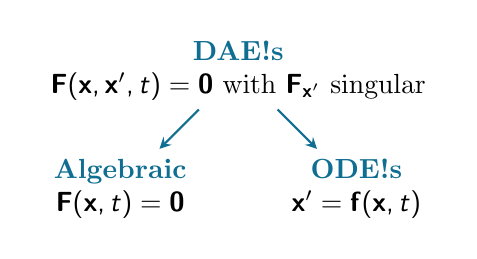
\begin{tikzpicture}[scale=0.5]
        \node at (0,0) {%
          $\begin{array}{c}%
          \text{\hi{\acsp{DAE}}} \\%
          \mF = \m{0}~\text{with $\m{F}_{\mxp}$ singular}%
          \end{array}$%
        };
        \draw[fg_sl_color, thick, -stealth] (-1,-1) -- (-2,-2);
        \node at (-3,-3) {%
          $\begin{array}{c}%
            \text{\hi{Algebraic}} \\
              \m{F}(\mx, t) = \m{0}
          \end{array}$%
        };
        \draw[fg_sl_color, thick, -stealth] (+1,-1) -- (+2,-2);
        \node at (+3,-3) {%
          $\begin{array}{c}%
            \text{\hi{\acsp{ODE}}} \\
            \mxp = \m{f}(\mx, t)
          \end{array}$%
        };
        \end{tikzpicture}}
        \item composed of
        \begin{itemize}
          \item<2-> differential equations describe the system's \textbf{dynamics}
          \item<2-> algebraic equations constrain the system to a \textbf{manifold} \\
        \end{itemize}
      \end{enumerate}
    \end{column}
    \begin{column}{0.35\textwidth}
      \centering
      \small
      \uncover<2->{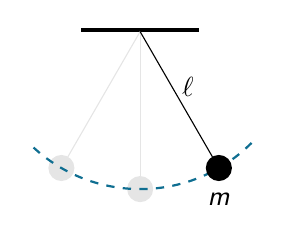
\begin{tikzpicture}[scale=0.5]
        \fill (-1.5,0) rectangle (1.5,0.1);
        \draw[tx_sl_color!10] (0,0) -- (-90:4) node [fill, circle]{};
        \draw[tx_sl_color!10] (0,0) -- (-120:4) node [fill, circle]{};
        \draw[fg_sl_color, thick, dashed] (2.8284, -2.8284) arc (-45:-135:4);
        \draw (0,0) -- (-60:4) node[fill, circle](m){};
        \node at (m) [below, yshift=-2mm] {$m$};
        \node at (1.2142, -1.4142) {$\ell$};
      \end{tikzpicture}
      \begin{equation*}
        \begin{array}{c}
          \text{\acs{ODE}} \\ \text{model}
        \end{array}
        \begin{cases}
          \theta^\prime = \omega \\
          \omega^\prime = -\dfrac{g}{\ell} \sin(\theta)
        \end{cases}
      \end{equation*}
      \begin{equation*}
        \begin{array}{c}
          \text{\acs{DAE}} \\ \text{model}
        \end{array}
        \begin{cases}
          x^\prime = u \\
          y^\prime = v \\
          u^\prime = -2x\lambda \\
          v^\prime = -2y\lambda - gm \\
          \, \textcolor{fg_sl_color}{0 = x^2 + y^2 - \ell^2}
        \end{cases}
      \end{equation*}}
    \end{column}
  \end{columns}
\end{frame}

\subsection{Solution of \aclp{DAE}}

\begin{frame}{Solution of \aclp{DAE}}{\acsp{DAE} are not \acsp{ODE}}
  Is the solution of \acsp{DAE} a straightforward extension of \acsp{ODE}?
  \begin{itemize}
    \item<1,3-> Specialized \textbf{numerical techniques} are required
    \item<2-> \textbf{Reformulation} of the \acs{DAE} system is typically required
  \end{itemize}
  \vspace{1.0em}
  \centering
  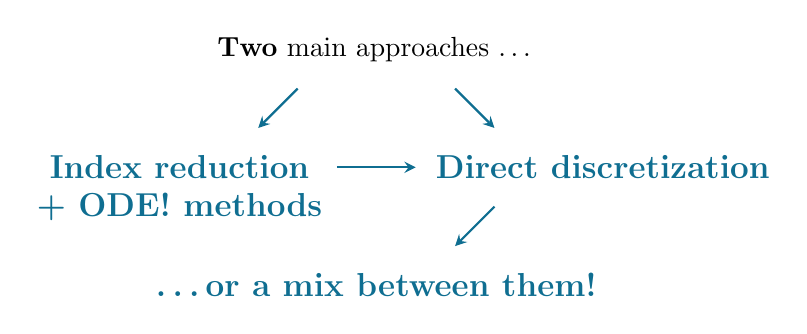
\begin{tikzpicture}[scale=0.5]
    \uncover<1->{\node at (0,0) {\textbf{Two} main approaches \dots};}
    \visible<2->{\draw[fg_sl_color, thick, -stealth] (-2,-1) -- (-3,-2);}
    \uncover<2->{\node at (-5,-3) {\hi{\large Index reduction}};}
    \visible<2>{\node at (-5,-4) {\hi{\large + \acs{ODE} methods}};}
    \visible<1>{\draw[fg_sl_color, thick, -stealth] (+2,-1) -- (+3,-2);}
    \uncover<1,3->{\node at (+5.75,-3) {\hi{\large Direct discretization}};}
    \visible<3->{
      \node at (0,-6) {\hi{\large \dots or a mix between them!}};
      \draw[fg_sl_color, thick, -stealth] (-1,-3) -- (+1,-3);
      \draw[fg_sl_color, thick, -stealth] (+3,-4) -- (+2,-5);
    }
  \end{tikzpicture} \\[0.5em]
  \uncover<1->{\raggedright\scriptsize{\fullcite{petzold1982differential}}}
\end{frame}

\subsubsection{Direct Discretization}

\begin{frame}{Solution of \aclp{DAE}}{Direct Discretization}
  \begin{itemize}[<+->]
    \item Approximate $\mxp$ through a \textbf{discretization formula} \\
    \begin{small}
      \qquad finite difference scheme \\
      \qquad polynomial quadrature
    \end{small}
    %\item This discretization can be written as an \textbf{implicit Runge-Kutta} method
    \begin{equation*}
      \begin{array}{c}
        \text{Implicit} \\
        \text{Runge-Kutta}
      \end{array}
      \quad
      \begin{array}{l}
        \m{F}\left(\m{x}_{k} + h_k\displaystyle\sum_{j=1}^{s}a_{ij} \m{K}_j, \m{K}_i, t_{k} + c_i h_k\right) = \m{0} \\[0.5em]
        \m{x}_{k+1} = \m{x}_{k} + h_k\displaystyle\sum_{i=1}^{s} b_i \m{K}_i
      \end{array}
      \quad \text{for} \quad
      \begin{array}{l}
        i = 1, \dots, s \\
        k = 0, 1, \dots, m
      \end{array}
    \end{equation*}
    $(a_{ij})$ non-singular + $h_k$ small enough $\rightarrow$ we can solve for $\m{K}_i$ at each $m$-th step
    \item[\textcolor{mycolor3}{\faExclamationTriangle}] Some \textbf{order of convergence} can be lost on some components depending on the \textcolor{mycolor2!95!black}{\textbf{index}}
  \end{itemize}
  \vspace{0.5em}
  \uncover<1->{\scriptsize{\fullcite{gear1971simultaneous}}}
\end{frame}

\subsubsection{Index Reduction}

\begin{frame}{Solution of \aclp{DAE}}{The Index \dots Or better Yet, The Indices}
  The index is a ``\textbf{measure of difficulty}'' in the solution of the \acsp{DAE} \dots
  \begin{itemize}
    \item Different approaches in classifying such difficulties led to different \textbf{index concepts} \\
    \centering{\small\begin{tabular}{ccc}
      \hi{differential} & structural & tractability \\
      geometrical & perturbation & strangeness
    \end{tabular}}
    \item \raggedright Some indices \textbf{coincide} under proper regularity conditions
  \end{itemize}
  \vspace{0.25em}
  \uncover<2->{\begin{bbox}[The Differential Index]
    It is the minimum number of differentiations required to transform a \acs{DAE} system into its underlying \acs{ODE} system.
  \end{bbox}}
  \vspace{0.25em}
  \scriptsize{\fullcite{mehrmann2015index}}
\end{frame}

\begin{frame}{Solution of \aclp{DAE}}{Index Reduction}
  \begin{bbox}[Index Reduction in the Solution Process]
    \vspace{-1.0em}
    \begin{equation*}
      \begin{array}{c}
        \text{High-index} \\
        \text{\acs{DAE}}
      \end{array}
      \quad \autorightarrow{\text{index}}{\text{reduction}} \quad
      \begin{array}{c}
        \text{\acs{ODE}} \\
        \text{or} \\
        \text{Index-1 \acs{DAE}} \\
      \end{array} {\!+~\text{Invariants}}
      \quad \autorightarrow{\text{numerical}}{\text{integration}} \quad
      \begin{array}{c}
        \text{Solution of} \\
        \text{original \acs{DAE}}
      \end{array}
    \end{equation*}
  \end{bbox}
  \vspace{1.0em}
  Index reduction is performed \dots
  \begin{itemize}
    \item \textbf{prior} to numerical integration
    \item by expressions \textbf{manipulation} and \textbf{differentiation}
    \item through \textbf{symbolic computation} or \textbf{numerically} (with \emph{automatic differentiation})
  \end{itemize}
  \vspace{0.5em}
    \hic{No simple recipe exists!}
  \centering{\small\begin{tabular}{cc}
    Structural methods & Projector-based analysis
  \end{tabular}}
\end{frame}

\begin{frame}{Solution of \aclp{DAE}}{Differential and Algebraic Equations Separation}
  \uncover<1->{\hic{How do we reduce the index?}
  Exploit an idea common to many index concepts!
  \begin{enumerate}
    \item \textbf{Separate} the differential and algebraic equations
    \item \textbf{Differentiate} the algebraic equations
    \item \textbf{Repeat} \boxednumber{1}--\boxednumber{2} until necessary (index-1 \acs{DAE} or \acs{ODE} is reached)
  \end{enumerate}}
  \vspace{0.5em}
  \uncover<2->{\centering{Easy to say, not so easy to do \dots} \\
  \vspace{0.5em}
  \setlength{\tabcolsep}{3.5em}
  \small\begin{tabular}{cc}
    \hi{Numerically}                                             & \hi{Symbolically} \\
    \textcolor{mycolor5!95!black}{Numerical linear algebra}      & \textcolor{mycolor2!95!black}{Symbolic linear algebra} \\
    \textcolor{mycolor3!95!black}{Automatic differentiation}     & \textcolor{mycolor5!95!black}{Symbolic differentiation} \\
    \textcolor{mycolor2!95!black}{Track of the separators chain} & \textcolor{mycolor5!95!black}{Just manipulate the equations}
  \end{tabular}} \\[0.5em]
  \uncover<1->{\raggedright\scriptsize{\fullcite{mehrmann2015index}}}
\end{frame}

\subsection{A New Algorithm for Index Reduction}

\begin{frame}{Solution of \aclp{DAE}}{A New Algorithm for Index Reduction}
  \uncover<1->{\hic{How can we improve the state-of-the-art?}
  Exploit the \textbf{equation separation} concept in a \textbf{full-symbolic} framework!
  \begin{itemize}
    \item[\raisebox{-1pt}{\scalebox{0.8}{\faQuestion}}] \textbf{No} a priori knowledge of the system structure
    \item[\raisebox{-1pt}{\scalebox{0.8}{\faPaperPlane}}] \textbf{Basic} use of symbolic computation and linear algebra
  \end{itemize}
  \vspace{0.5em}
  \begin{columns}
    \centering
    \begin{column}[t]{0.25\textwidth}
      \centering
      \hi{Differentiation} \\[0.25em]
      $\dfrac{\text{d}}{\text{d}\textbf{x}}$ \vspace*{0.15cm}
    \end{column}
    \begin{column}[t]{0.25\textwidth}
      \centering
      \hi{Factorization} \\
      LU \\ Fraction-Free LU
    \end{column}
  \end{columns}}
  \vspace{0.5em}
  The tools we are going to use are \dots \\
  \begin{itemize}\small
    \item[\raisebox{0pt}{\scalebox{1.0}{\faCanadianMapleLeaf}}] \textbf{\Maple{}} for symbolic manipulation \\
    \item[\raisebox{0pt}{\scalebox{0.8}{\faAngleRight\hspace{-0.1em}\faAngleRight\hspace{-0.1em}\faAngleRight}}] \textbf{\Matlab{}} for numerical evaluation
  \end{itemize}
\end{frame}

% That's all Folks!

%!TEX root = main.tex

\section{Symbolic Computation Essentials}

\subsection{Expression Swell}

\begin{frame}{Symbolic Computation Essentials}{Expression Swell}
  \uncover<1->{\begin{center}\begin{minipage}{\textwidth}\begin{bbox}[Inside a \acs{CAS}]
    \centering%
    \begin{minipage}[c]{0.15\textwidth} \centering Input expression \end{minipage}%
    \begin{minipage}[c]{0.19\textwidth} \centering $\autorightarrow{\text{symbolic}}{\text{manipulation}}$ \end{minipage}%
    \begin{minipage}[c]{0.21\textwidth} \centering Output expression \\ + \\ Expression swell \end{minipage}%
    \begin{minipage}[c]{0.19\textwidth} \centering $\autorightarrow{\text{symbolic}}{\text{simplification}}$ \end{minipage}%
    \begin{minipage}[c]{0.23\textwidth} \centering Output expression \\ \visible<2->{+ \\ \textcolor{mycolor2!95!black}{Expression swell}}\end{minipage}%
  \end{bbox}\end{minipage}\end{center}}
  \uncover<2->{\hic{\acs{CAS} are sensitive to expression swell!}
  \centering{\small\begin{tabular}{cc}
    \textcolor{fg_sl_color}{\faCoins} High memory usage & Slow computation \textcolor{fg_sl_color}{\faHourglassHalf}
  \end{tabular}}} \\[0.5em]
  \centering{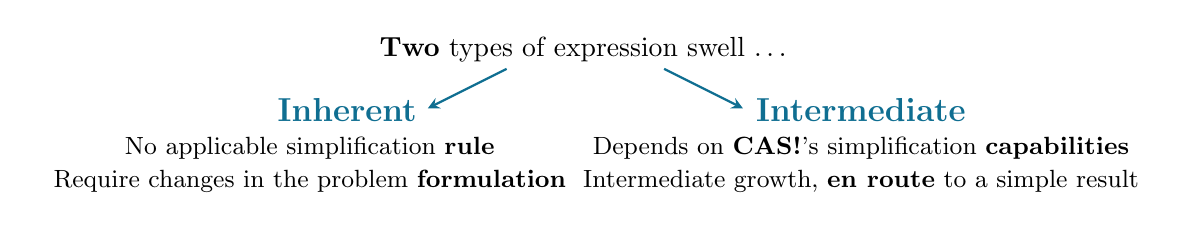
\begin{tikzpicture}[scale=0.5]
    \uncover<3->{
      \node at (0,0) {\textbf{Two} types of expression swell \dots};
      \draw[fg_sl_color, thick, -stealth] (-2,-0.5) -- (-4.0,-1.5);
      \node at (-7,-2.5) {
      \begin{tabular}{c}
        \hi{\large ~~~~~~Inherent} \\
        \small{No applicable simplification \textbf{rule}} \\
        \small{Require changes in the problem \textbf{formulation}}
      \end{tabular}};
    }
    \uncover<4->{\draw[fg_sl_color, thick, -stealth] (+2,-0.5) -- (+4.0,-1.5);
    \node at (+7,-2.5) {
      \begin{tabular}{c}
        \hi{\large Intermediate} \\
        \small{Depends on \acs{CAS}'s simplification \textbf{capabilities}} \\
        \small{Intermediate growth, \textbf{en route} to a simple result}
      \end{tabular}
    };}
  \end{tikzpicture}}
\end{frame}

\subsection{\acl{LEM}}

\begin{frame}{\acl{LEM}}{Hierarchical Representation}
  We progressively \textbf{hide} chuncks of expressions
  \begin{equation*}
    \begin{array}{c}
      \textcolor{mycolor1}{\underline{2xy(1+y)}} \cdot f(x,y) + \textcolor{mycolor2}{\underline{5z(3a+z)}} \cdot g(y) + \textcolor{mycolor3}{\underline{3c(xy+z)}} \cdot h(x,z) \\[0.1em]
      \textcolor{mycolor5}{\underline{v_1 \cdot f(x,y)}} + \textcolor{mycolor4}{\underline{v_2 \cdot g(y) + v_3 \cdot h(x,z)}} \\[0.1em]
      v_4 + v_5
    \end{array}
  \end{equation*}
  to store them in separate variables
  \begin{align*}
    \textcolor{mycolor1}{v_1} &= 2x(1+y) \\
    \textcolor{mycolor2}{v_2} &= 5z(3a+z) \\
    \textcolor{mycolor3}{v_3} &= 3c(xy+z) \\
    \textcolor{mycolor4}{v_4} &= \textcolor{mycolor1}{v_1} \cdot f(x,y) \\
    \textcolor{mycolor5}{v_5} &= \textcolor{mycolor2}{v_2} \cdot g(y) + \textcolor{mycolor3}{v_3} \cdot h(x,z)
  \end{align*}
\end{frame}

\begin{frame}{\acl{LEM}}{Hierarchical Representation}
  \uncover<1->{\textbf{Hierarchical representation} of expressions is performed through \textbf{veiling variables}
  \begin{equation*}
    \m{f}(\mx) \quad \autorightarrow{\text{veiling}}{\text{variables}} \quad \m{f}(\mx, \m{v})
    \qquad \text{where} \qquad
    \m{v}(\mx) = \msmall{\begin{bmatrix}
      v_{1}(\mx) \\
      v_{2}(v_{1}, \mx) \\
      \vdots \\
      v_{n}(v_{1}, \dots, v_{n-1}, \mx)
    \end{bmatrix}}
  \end{equation*}}
  \uncover<2->{\textbf{\acs{LEM}} is made of two actions \dots
  \begin{enumerate}
    \item \textbf{veiled} large expressions
    \item \textbf{unveil} to recover the original form
  \end{enumerate}}
  \vspace{0.5em}
  \uncover<3->{\hic{Complexity remains but the \acs{CAS} can not see it! \textcolor{fg_sl_color}{\large \faGlasses}}}
\end{frame}

\begin{frame}{\acl{LEM}}{Measuring Expression Complexity}
  \centering{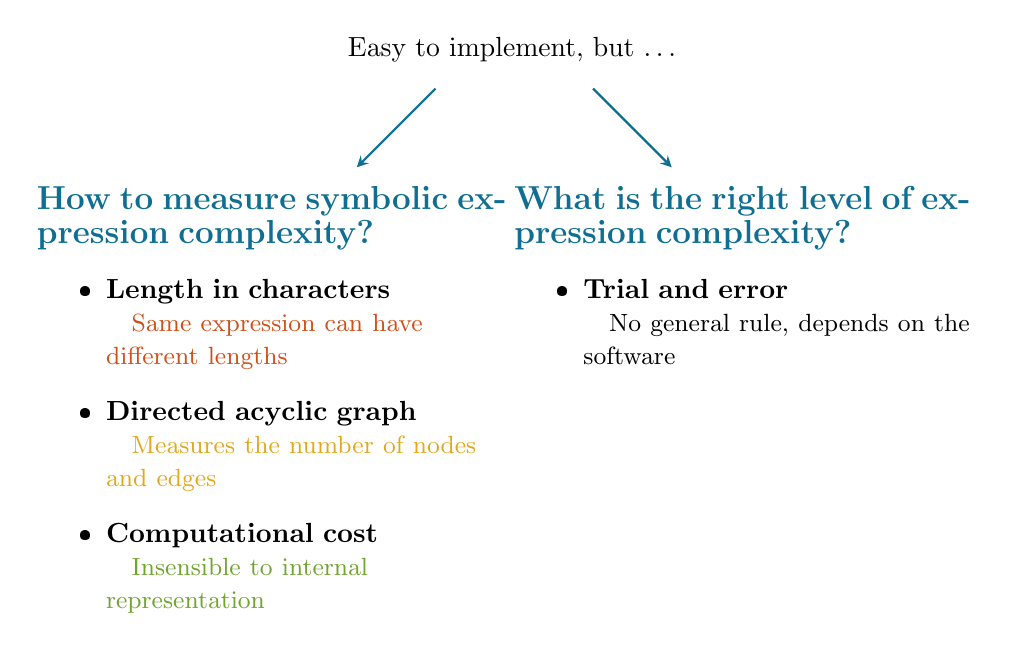
\begin{tikzpicture}[scale=0.5]
    \node at (0,0) {Easy to implement, but \dots};
    \uncover<1->{
      \draw[fg_sl_color, thick, -stealth] (-2,-1) -- (-4.0,-3);
      \draw (-0.5\textwidth,-3.25) node[below, text width=0.5\textwidth] {
      \hi{\large How to measure symbolic expression complexity?}
      \begin{itemize}
        \item \textbf{Length in characters} \\
        \begin{small}
          \quad \textcolor{mycolor2!95!black}{Same expression can have different lengths}
        \end{small}
        \item \textbf{Directed acyclic graph} \\
        \begin{small}
          \quad \textcolor{mycolor3!95!black}{Measures the number of nodes and edges}
        \end{small}
        \item \textbf{Computational cost} \\
        \begin{small}
          \quad \textcolor{mycolor5!95!black}{Insensible to internal representation}
        \end{small}
      \end{itemize}
    };}
    \uncover<2->{
      \draw[fg_sl_color, thick, -stealth] (+2,-1) -- (+4.0,-3);
      \draw (0.5\textwidth,-3.25) node[below, text width=0.5\textwidth] {
      \hi{\large What is the right level of expression complexity?}
      \begin{itemize}
        \item \textbf{Trial and error} \\
        \begin{small}
          \quad No general rule, depends on the software
        \end{small}
      \end{itemize}};
    }
  \end{tikzpicture}}
\end{frame}

\subsection{Symbolic Matrix Factorization}

\begin{frame}{Symbolic Matrix Factorization}{Considerations and Challenges}
  \hic{\faCanadianMapleLeaf~\Maple{} factorizations are sensitive to expression swell}
  \begin{itemize}
    \item<2-> \textbf{\acl{LU}~(\acs{LU})} and \textbf{\acl{FFLU}~(\acs{FFLU})} factorizations \dots \\
    \begin{small}
      \qquad preserve \textbf{sparsity} and \textbf{fill-in} \\
      \qquad perform \textbf{minimal algebraic manipulations} \\
      \qquad allow for custom \textbf{pivoting strategies}
    \end{small}
  \item<3->However\dots
    \begin{enumerate}
      \normalsize
      \item output's numerical stability is not guaranteed \\
      \begin{small}
        \qquad \textbf{How to ensure numerical stability?}
      \end{small}
      \item expressions grow unpredictably during manipulation \\
      \begin{small}
        \qquad \textbf{How to manage large symbolic expressions?}
      \end{small}
    \end{enumerate}
  \end{itemize}
\end{frame}

\begin{frame}{Symbolic Matrix Factorization}{Symbolic Pivoting Strategy}
  \vspace{-1.5em}
  \hic{How to ensure numerical stability?}
  \begin{columns}
    \begin{column}[c]{0.47\textwidth}
      A good symbolic \textbf{pivoting strategy} \dots
      \begin{enumerate}
        \item<1> selects the \textbf{minimum-degree} entry \\
        \begin{small}
          \qquad Limit fill-in and expression swell
        \end{small}
        \item<2> if numeric, selects the \textbf{biggest} entry \\
        \begin{small}
          \qquad Improve numerical stability
        \end{small}
        \item<3> selects \textbf{least complicated} entry \\
        \begin{small}
          \qquad Limit expression swell
        \end{small}
        \item<4> looks for the \textbf{best choice} \\
        \begin{small}
          \qquad Full-pivoting strategy
        \end{small}
      \end{enumerate}
    \end{column}
    \begin{column}[c]{0.53\textwidth}
      \begin{algorithmic}\scriptsize
        \Procedure{SymbolicPivoting}{$\m{A}$, $k$}
        \State \only<1>{\hlc}{$\m{d}^r, \, \m{d}^c \gets \text{ComputeDegrees}(\m{A})$}
          \For{\only<4>{\hlc}{$i$ \textbf{from} $k$ \textbf{to} $m$}}
          \For{\only<4>{\hlc}{$j$ \textbf{from} $k$ \textbf{to} $n$}}
              \State $D_{ij} \gets \infty$
              \IfThen{$A_{ij} \neq 0$}
              {\only<1>{\hlc}{$D_{ij} \gets d^r_{i} \, \max(0, \, d^c_j-1) + d^c_j \, \max(0, \, d^r_i-1)$}}
            \EndFor
          \EndFor
          \State \only<1>{\hlc}{$\mathcal{P} \gets \text{Sort}(\m{D})$}
          \State $q, \, l \gets \, 0, \, 0$  and $p, \, p_c, \, p_n \gets \infty, \, \infty, \, \infty$
          \For{\textbf{all} $(i, j)$ \textbf{in} $\mathcal{P}$}
            \IfThen{$p_c \neq \infty$ \textbf{and} $D_{ij} > D_{ql}$}{\textbf{break}}
            \State $t \gets A_{ij}$
            \IfThen{$\text{Signature}(t) = 0$}{\textbf{continue}}
            \State $t \gets \text{Simplify}(t)$ and \only<3>{\hlc}{$t_c \gets \text{ExpressionComplexity}(t)$} and $t_n \gets \infty$
            \IfThen{$t$ is numeric}{\only<2>{\hlc}{$t_n \gets \max(1, \, \text{abs}(t))$}}
            \If{\only<3>{\hlc}{$t_c < p_c$} \textbf{or} (\only<2>{\hlc}{$t_c = p_c$} \textbf{and} \only<2>{\hlc}{$t_n > p_n$})}
              \State $q, \, l \gets i, \, j$ and $p, \, p_c, \, p_n \gets t, \, t_c, \, t_n$
            \EndIf
          \EndFor
          \State \textbf{return} $p, \, q, \, l$
        \EndProcedure
      \end{algorithmic}
    \end{column}
  \end{columns}
\end{frame}

\begin{frame}{Symbolic Matrix Factorization}{\acs{LEM} During Factorization}
  \vspace{-1.5em}
  \hic{How to manage large symbolic expressions?}
  \begin{columns}
    \begin{column}[c]{0.32\textwidth}
      Veils are introduced during \dots
      \begin{itemize}
        \item<1> \textbf{Factorization step} \\
        \begin{small}
          \qquad gaussian elimination \\
          \qquad Schur complement
        \end{small}
        \item<2> \textbf{Solution step} \\
        \begin{small}
          \qquad forward substitution \\
          \qquad backward substitution
        \end{small}
      \end{itemize}
    \end{column}
    \begin{column}[c]{0.36\textwidth}
      \uncover<1>{\begin{algorithmic}\scriptsize
        \Procedure{LU}{$\m{A}, \, k$}
          \State $\m{M} \gets \m{A}$
          \State $rnk \gets \min(m, \, n)$
          \For{$k$ \textbf{from} $1$ \textbf{to} $rnk$}
            \State $p, \, q, \, l \gets \text{SymbolicPivoting}(\m{M}, \, k)$
            \If{$p = 0$}
              \State $rnk \gets k-1$ and \textbf{break}
            \EndIf
            \State $\m{r}_k, \, \m{c}_k \gets \, q, \, l$
            \State $\m{M} \gets \text{SwapRowsCols}(\m{M}, \, k, \, q,  \, l)$
            \For{$i$ \textbf{from} $k+1$ \textbf{to} $m$}
              \State \only<1>{\hlc}{$M_{kk} \gets \text{Veil}(M_{kk})$}
              \State \only<1>{\hlc}{$M_{ik} \gets \text{Veil}(\text{Normalizer}(M_{ik}/M_{kk}))$}
              \For{$j$ \textbf{from} $k+1$ \textbf{to} $n$}
                \State \only<1>{\hlc}{$M_{ij} \gets \text{Veil}(\text{Normalizer}(M_{ij} - M_{ik}M_{kj}))$}
              \EndFor
            \EndFor
          \EndFor
          \State $\m{P}, \, \m{Q} \gets \text{PermutationMatrices}(\m{r}, \, \m{c})$
          \State $\m{L}, \, \m{U} \gets \text{LowerUpperMatrices}(\m{M})$
          \State \textbf{return} $\m{L}, \, \m{U}, \, \m{P}, \, \m{Q}, \, \m{r}, \, \m{c}, \, rnk$
        \EndProcedure
      \end{algorithmic}}
    \end{column}
    \begin{column}[c]{0.32\textwidth}
      \uncover<2>{\begin{algorithmic}\scriptsize
        \Procedure{SolveLU}{$\m{L}, \, \m{U}, \, \m{P}, \, \m{Q}, \, \m{b}$}
          \State $\m{y} \gets \m{P}\m{b}$
          \State $m, \, n \gets \text{Size}(\m{L})$
          \For{$i$ \textbf{from} $2$ \textbf{to} $m$}
            \State \only<2>{\hlc}{$y_i \gets \text{Veil}(y_i - \sum\nolimits_{j=1}^{i-1} L_{ij}y_j)$}
          \EndFor
          \State $x_n \gets \text{Veil}(y_n/U_{nn})$
          \For{$i$ \textbf{from} $n-1$ \textbf{to} $1$}
            \State \only<2>{\hlc}{$x_i \gets \text{Veil}(y_i - {\sum\nolimits_{j=i+1}^{n}} U_{ij}x_j)$}
            \State \only<2>{\hlc}{$x_i \gets \text{Veil}(x_i/U_{ii})$}
          \EndFor
          \State $\m{x} \gets \m{Q}^\top\m{x}$
        \EndProcedure
      \end{algorithmic}}
    \end{column}
  \end{columns}
\end{frame}

% That's all Folks!

%!TEX root = main.tex

\section{Index Reduction Algorithm}

\subsection{Separation of Differential and Algebraic Equations}

\begin{frame}{Index Reduction Algorithm}{Separation of Differential and Algebraic Equations}
  \vspace{-1.0em}
  \begin{columns}
    \begin{column}[c]{0.6\textwidth}
      \begin{enumerate}[<+->]
        \item Consider the \textbf{generic} \acsp{DAE} system
        \begin{equation*}
          \mF = \mA \mxp - \mb = \m{0}
        \end{equation*}
        \item \textbf{Separate} the equations with the cokernel $\mK$ and its orthogonal complement $\mN$ of $\mA$
        \begin{equation*}
          \begin{bmatrix} \mE \\ \m{0} \end{bmatrix} \mxp = \begin{bmatrix} \mg \\ \ma \end{bmatrix}
          ~~ \text{with} ~~
          \begin{array}{r@{~}c@{~}l}
            \mE &=& \mN \mA \\
            \mg &=& \mN \mb \\
            \ma &=& \mK \mb
          \end{array}
        \end{equation*}
      \end{enumerate}
      \vspace{-1.0em}
      \uncover<3->{\begin{bbox}[Cokernel Computation]
        The cokernel $\mK$ and its orthogonal complement $\mN$ of $\mA$ are calculated using matrix factorization
      \end{bbox}}
    \end{column}
    \begin{column}[c]{0.4\textwidth}
      \visible<3->{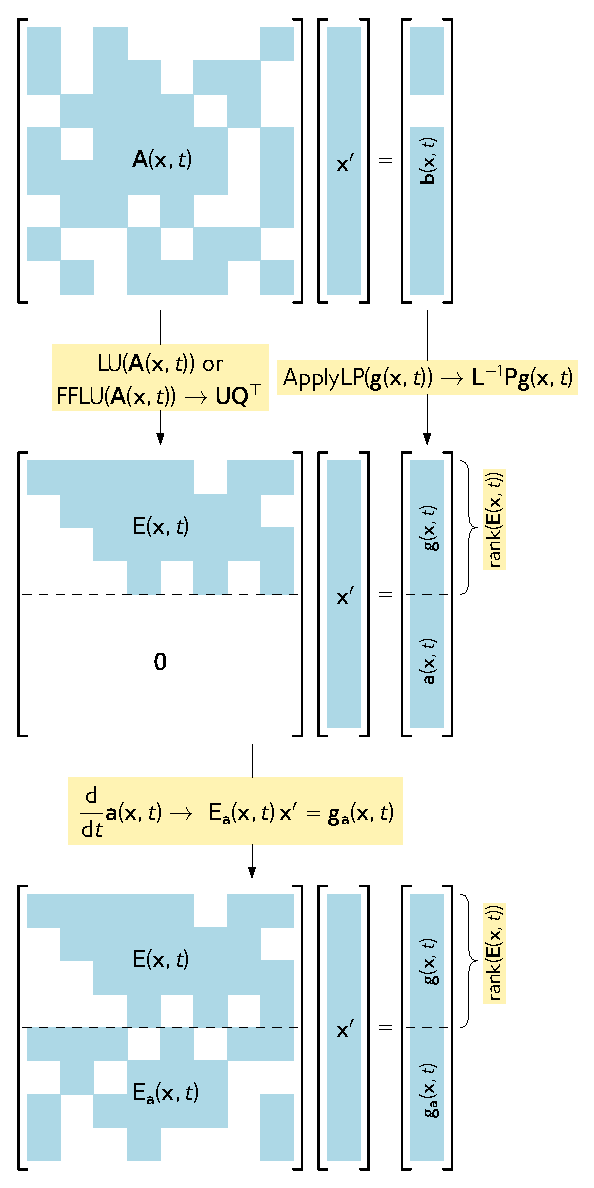
\includegraphics[width=1.0\textwidth, trim={0cm 7.35cm 0cm 0cm}, clip]{dae_visualization.eps}}
    \end{column}
  \end{columns}
\end{frame}

\subsection{Differentiation of Algebraic Equations}

\begin{frame}{Index Reduction Algorithm}{Differentiation of Algebraic Equations}
  \vspace{-1.5em}
  \begin{columns}
    \begin{column}[c]{0.6\textwidth}
      \begin{enumerate}[<+->]\setcounter{enumi}{2}
        \item Update the \textbf{invariants} as $\mh = \mh \cup \ma$
        \item \textbf{Differentiate} the algebraic equations $\ma$
        \begin{equation*}
          \dfrac{\text{d}}{\text{d}t} \ma = \mAd \mxp - \mgd
        \end{equation*}
        \item The \textbf{index reduced} system of \acsp{DAE} takes the form
        \begin{align*}
          \mF = \mA &\mxp - \mb = \m{0} ~~ \text{with} \\
          \mA = \begin{bmatrix} \mE \\ \mAd \end{bmatrix}
          ~~ &\text{and} ~~
          \mb = \begin{bmatrix} \mg \\ \mgd \end{bmatrix}
        \end{align*}
      \end{enumerate}
      \uncover<3->{\begin{bbox}[A Sequential Algorithm]
        Apply \boxednumber{1}--\boxednumber{6} repeatedly until $\mA$ is non-singular
      \end{bbox}}
    \end{column}
    \begin{column}[c]{0.4\textwidth}
      \visible<2->{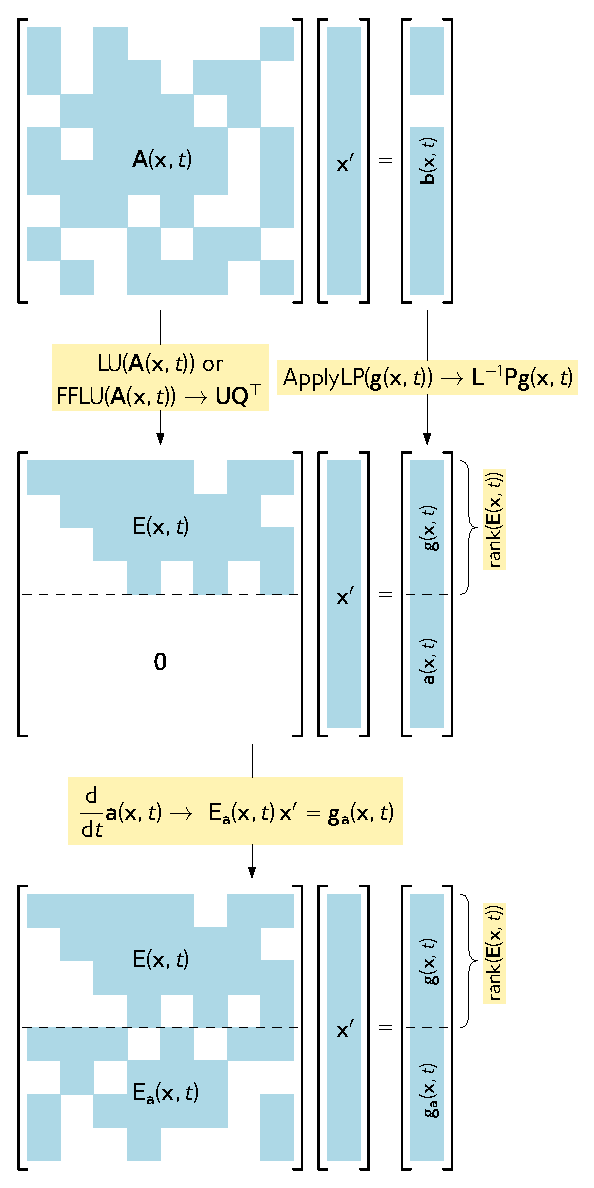
\includegraphics[width=1.0\textwidth, trim={0cm 0cm 0cm 7.35cm}, clip]{dae_visualization.eps}}
    \end{column}
  \end{columns}
\end{frame}

\begin{frame}{Index Reduction Algorithm}{Including Veiling Variables}
  \vspace{-1.0em}
  The algorithm can be extended to include \textbf{\acs{LEM}}
  \begin{itemize}
    \item veiling variables are stored in the list $\mv$
    \item equations are also function of $\mv$
    \item veiling variables add an evaluation layer to the algorithm
  \end{itemize}
  \vspace{-1.5em}\hspace{-0.025\textwidth}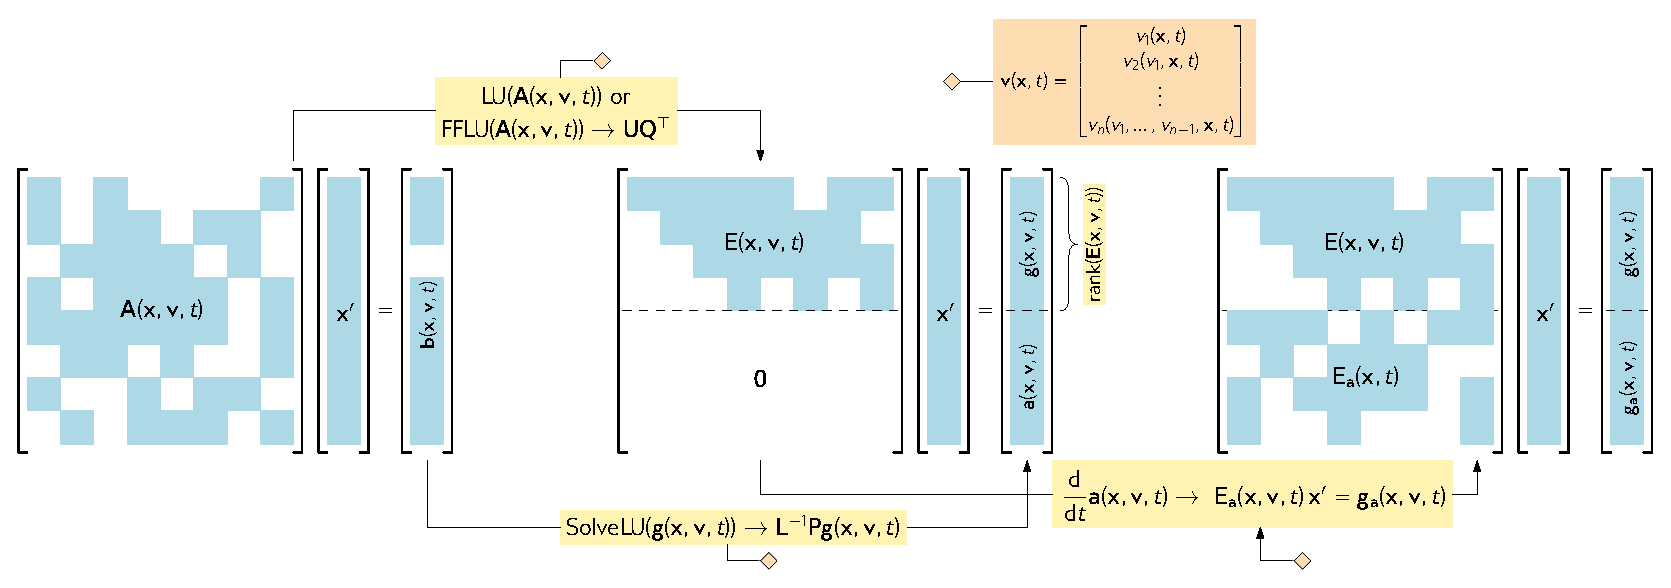
\includegraphics[width=1.05\textwidth]{dae_visualization_veil.eps}
\end{frame}

%\begin{frame}{Index Reduction Algorithm}{Algorithm Flowchart}
%  \centering
%  \begin{tikzpicture}[overlay]
%    \node at (0,0) {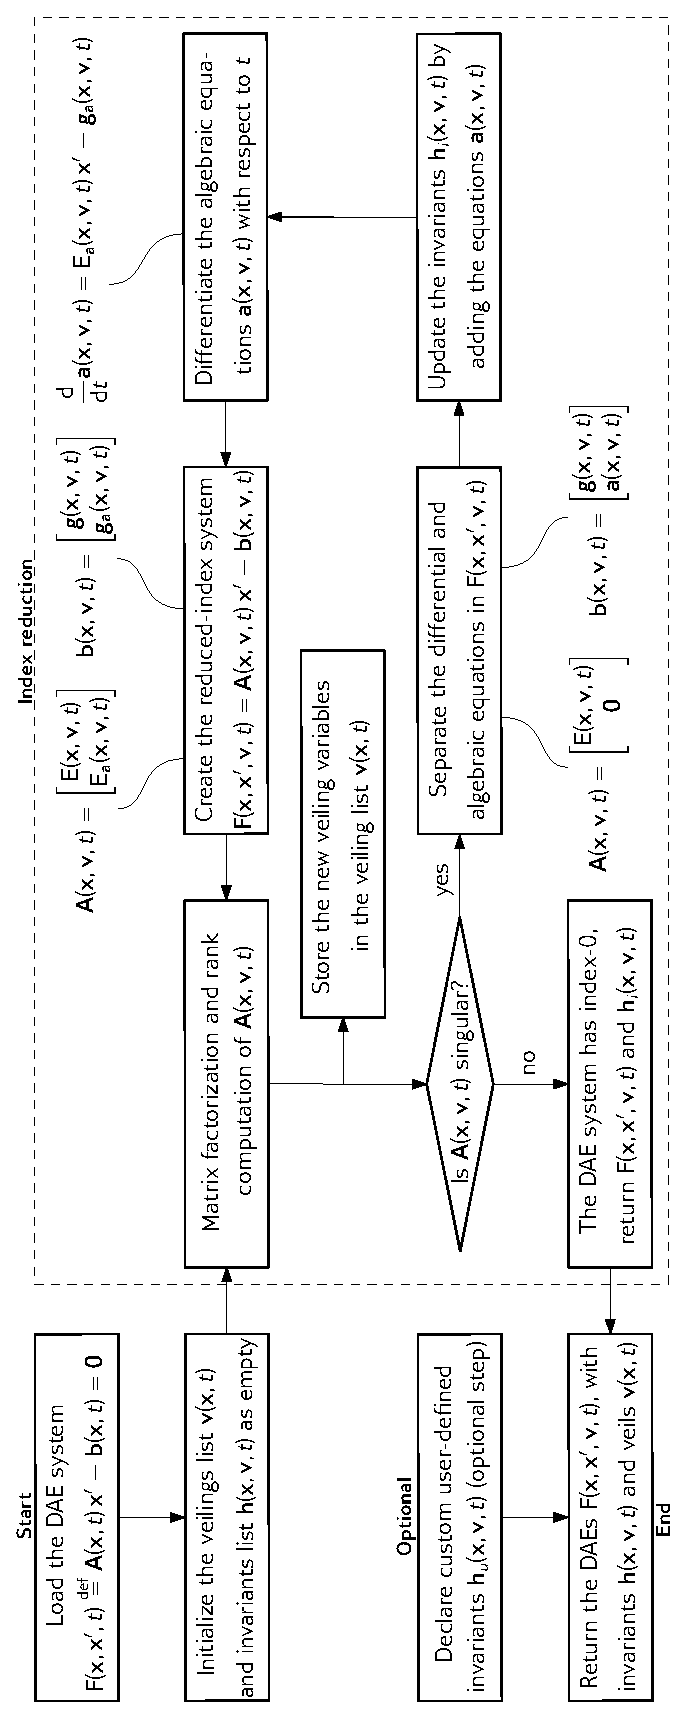
\includegraphics[angle=270, width=1.0\textwidth]{dae_flowchart_veil}};
%    \only<1>{\draw[fg_sl_color, line width=1.0pt] (-7.2,  2.9) rectangle (-3.7,  0.4);} % Initialization
%    \only<2>{\draw[fg_sl_color, line width=1.0pt] (-3.7,  2.9) rectangle ( 7.2, -2.9);} % Index Reduction
%    \only<3>{\draw[fg_sl_color, dashed, line width=1.0pt] (-7.2, -0.3) rectangle (-3.7, -1.6);} % Optional step
%    \only<4>{\draw[fg_sl_color, line width=1.0pt] (-7.2, -1.6) rectangle (-3.7, -2.9);} % Finalization
%  \end{tikzpicture}
%\end{frame}

\begin{frame}{Index Reduction Algorithm}{The Reduced \acs{DAE} System}
  \vspace{-1.0em}
  \hic{\faCanadianMapleLeaf~Now we can code-generate the reduced \acs{DAE} system!}
  \begin{itemize}[<+->]
    \item \textbf{Differential part}
    %
    \begin{equation*}
      \begin{array}{ccl}
          \m{F}(\mx, \mx^\prime, \m{v}, t) = \m{0} & \quad & \text{implicit  system class} \\
          \m{A}(\mx, \m{v}, t) \mx^\prime = \m{b}(\mx, \m{v}, t) & \quad & \text{semi-explicit system class} \\
          \mx^\prime = \m{f}(\mx, \m{v}, t) & \quad & \text{explicit system class}
      \end{array}
    \end{equation*}
    %
    \item \textbf{Invariants}
    %
    \begin{equation*}
      \m{h}(\mx, \m{v}, t) = \begin{bmatrix}
          \mhiv \\
          \mhuv
      \end{bmatrix} = \m{0} \quad \begin{array}{l}
        \text{hidden constraints} \\
        \text{\emph{optional} user-defined invariants}
        \end{array}
    \end{equation*}
    %
    \item \textbf{Veiling variables}
    %
    \begin{equation*}
        \m{v}(\mx, t) = \begin{bmatrix}
            v_{1}(\mx, t) \\
            v_{2}(v_{1}, \mx, t) \\
            \vdots \\
            v_{n}(v_{1}, \dots, v_{n-1}, \mx, t)
        \end{bmatrix}
    \end{equation*}
  \end{itemize}
\end{frame}

\subsection{Projection on Invariants}

\begin{frame}{Projection on Invariants}{Theoretical Background and Implementation}
  \vspace{-1.0em}
  \hic{\faAngleRight\hspace{-0.1em}\faAngleRight\hspace{-0.1em}\faAngleRight~Now we can integrate the system in \Matlab{}!}
  \begin{columns}
    \begin{column}[c]{0.6\textwidth}
      Projection is performed:
      \begin{itemize}
        \item during the \textbf{numerical integration}
        \item to \textbf{enforce} the solution $\mx$ onto the $\mhv$ manifold
        \item by solving the \textbf{constrained minimization} problem
          \begin{align*}
            \underset{\mx}{\text{minimize}} \quad &\dfrac{1}{2}\left(\mx - \tilde{\mx}\right)^2 \\
            \text{subject to} \quad &\mhv = \m{0}
          \end{align*}
        \end{itemize}
      \end{column}
      \begin{column}[c]{0.4\textwidth}
        \hspace{-0.2\textwidth}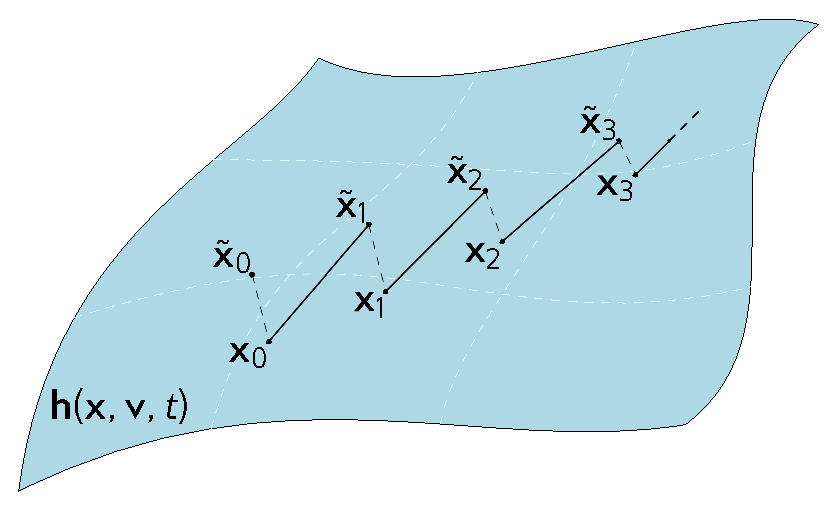
\includegraphics[width=1.2\textwidth]{projection.eps}
      \end{column}
    \end{columns}
    \vspace{1.0em}
    \hic{\large Find $\mx$ with minimal distance from $\tilde{\mx}$ that satisfies the invariants $\mhv$}
\end{frame}

%\begin{frame}{Projection on Invariants}{Theoretical Background and Implementation}
%  \begin{itemize}
%    \item The \textbf{Lagrangian} of the minimization problem is
%    \begin{equation*}
%      \mathcal{L}(\mx, \boldsymbol{\lambda}) = \frac{1}{2}\left(\mx - \tilde{\mx}\right)^2 + \boldsymbol{\lambda} \cdot \mhv
%      \quad \rightarrow \quad
%      \begin{cases}
%        \mx + \m{Jh}_\mx^\top \boldsymbol{\lambda} = \tilde{\mx} \\
%        \mhv = \m{0}
%      \end{cases}
%    \end{equation*}
%    \item The iterative method is \dots
%    \begin{equation*}
%      \begin{bmatrix}
%        \m{Jh}_{\mx} & \m{0} \\
%        \m{I}        & \m{Jh}_\mx^\top
%      \end{bmatrix}
%      \begin{bmatrix}
%        \delta\mx \\
%        \boldsymbol{\lambda}
%      \end{bmatrix} = \begin{bmatrix}
%        \tilde{\mx} - \mx \\
%        -\mhv
%      \end{bmatrix} \quad \text{where the step is} \quad \mx = \tilde{\mx} + \delta\mx
%    \end{equation*}
%    \item[] \dots derived from the \textbf{Taylor expansion}
%    \begin{equation*}
%      \begin{cases}
%        \mhv + \m{Jh}_{\mx}(\mx, \m{v}, t) \delta\mx + \textcolor{mycolor2}{\mathcal{O}\left(\| \delta\mx \|^2\right)} = \m{0} \\
%        \mx + \delta\mx + \m{Jh}_{\mx}^{\top}(\mx + \textcolor{mycolor2}{\delta \mx}, \m{v}, t) \boldsymbol{\lambda} = \tilde{\mx}
%      \end{cases}
%    \end{equation*}
%  \end{itemize}
%\end{frame}

\begin{frame}{Symbolic-Numerical Validation}{The Problem}
  \begin{columns}
    \begin{column}[c]{0.425\textwidth}
      A \textbf{particle} moving over a \textbf{torus} surface
      \begin{equation*}
        \begin{cases}
          x^{\prime}_{1} = u_{1} \\
          x^{\prime}_{2} = u_{2} \\
          x^{\prime}_{3} = u_{3} \\
          u^{\prime}_{1} = u_{3}\cos(t) - x_{3}\sin(t) - u_{2} + 2 c x_{1}\lambda \\
          u^{\prime}_{2} = u_{3}\sin(t) + x_{3}\cos(t) + u_{1} + 2 c x_{2}\lambda \\
          u^{\prime}_{3} = x_{3} + 2x_{3}\lambda \\
          \rho^2 = x_{1}^2 + x_{2}^2 + x_{3}^2 - 2r(x_{1}^2 + x_{2}^2)^{\frac{1}{2}} + r^2
        \end{cases}
      \end{equation*}
      with $c = 1 - r/(x_{1}^2 + x_{2}^2)^{\frac{1}{2}}$, $\rho = 5$, $r = 10$, and ICs $\mx_{0} = [15, 0, 0, 0, 15, -5, \lambda]^{\top}$
    \end{column}
    \begin{column}[c]{0.575\textwidth}
      \hic{\large Exact Solution}
      \begin{equation*}
        \mx_\text{exact} = \begin{bmatrix}
          x_{1} \\ x_{2} \\ x_{3}
        \end{bmatrix} = \begin{bmatrix}
          (\rho \cos(2\pi - t) + r) \cos(t) \\
          (\rho \cos(2\pi - t) + r) \sin(t) \\
          \rho \sin(2\pi - t)
        \end{bmatrix}
      \end{equation*} \\
      \centering{\includegraphics[width=0.6\textwidth, trim={17.0cm 3.5cm 2cm 2.5cm}, clip]{torus_3d_placeholder.png}}
    \end{column}
  \end{columns}
  \vspace{0.5em}
  \scriptsize{\fullcite{campbell1995constraint}}
\end{frame}

\begin{frame}{Symbolic-Numerical Validation}{Index Reduction}
  \vspace{-1.0em}
  \centering{\scriptsize\begin{tabular}{cccc}
    \multicolumn{4}{c}{\textbf{\acs{LU} Factorization}} \\
    \toprule
    \textbf{Original \acsp{DAE}} & \multicolumn{3}{c}{$\mF = 47\cf + 30\cm + 23\ca$ \quad $\mh = 0$} \\
    \midrule
    \textbf{Reduction step} & $\mE$ & $\mg$ & $\ma$ \\
    \midrule
    Index-3 \acsp{DAE} & $0$ & $39\cf + 36\cm + 13\ca$ & $7\cf + 10\cm + 6\ca$ \\
    Index-2 \acsp{DAE} & $0$ & $39\cf + 36\cm + 13\ca$ & $22\cf + 20\cm + 8\ca$ \\
    Index-1 \acsp{DAE} & $0$ & $39\cf + 36\cm + 13\ca$ & $68\cf + 72\cm + 33\ca$ \\
    Index-0 \acsp{DAE} & $388\cf + 424\cm + 180\ca$ & $79\cf + 77\cm + 26\ca$ & $0$ \\
    \midrule
    \rowcolor{mycolor5!25}
    \textbf{Reduced \acsp{DAE}} & \multicolumn{3}{c}{$\mF = 258\cf + 239\cm + 109\ca$ \quad $\mh = 97\cf + 102\cm + 47\ca$} \\
    \bottomrule \\[0.05em]
    %
    \multicolumn{4}{c}{\textbf{\acs{FFLU} Factorization}} \\
    \toprule
    \textbf{Original \acsp{DAE}} & \multicolumn{3}{c}{$\mF = 47\cf + 30\cm + 23\ca$ \quad $\mh = 0$} \\
    \midrule
    \textbf{Reduction step} & $\mE$ & $\mg$ & $\ma$ \\
    \midrule
    Index-3 \acsp{DAE} & $0$ & $39\cf + 36\cm + 13\ca$ & $7\cf + 10\cm + 6\ca$ \\
    Index-2 \acsp{DAE} & $0$ & $39\cf + 36\cm + 13\ca$ & $26\cf + 23\cm + 8\ca$ \\
    Index-1 \acsp{DAE} & $0$ & $39\cf + 36\cm + 13\ca$ & $68\cf + 72\cm + 33\ca$ \\
    Index-0 \acsp{DAE} & $388\cf + 424\cm + 180\ca$ & $79\cf + 77\cm + 26\ca$ & $0$ \\
    \midrule
    \rowcolor{mycolor2!25}
    \textbf{Reduced \acsp{DAE}} & \multicolumn{3}{c}{$\mF = 258\cf + 239\cm + 109\ca$ \quad $\mh = 101\cf + 105\cm + 47\ca$} \\
    \bottomrule \\[0.025em]
    \multicolumn{4}{c}{\small\emph{Legend}: $\cf$ = functions, $\ca$ = additions, $\cm$ = multiplications, and $\cd$ = divisions.}
    \end{tabular}}
\end{frame}

\begin{frame}{Symbolic-Numerical Validation}{Order and Error Analysis}
  \centering{\small{\input{figures/torus_order_hidden.tex}}}
\end{frame}

\begin{frame}{Symbolic-Numerical Validation}{Solution Visualization}
  \vspace{-1.0em}
  \hic{RadauIIA5 \quad $\Delta t = 0.05$\,s \quad $t \in [0, 200\pi]$\,s}
  \vspace{1.0em}
  \centering\small
  \textbf{No projection}%
  \hspace{10.0em}%
  \textbf{With projection}
  \movie[label=show1, width=0.8\textwidth, autostart, poster, showcontrols, loop]{\includegraphics[width=0.8\textwidth]{torus_3d_placeholder.png}}{movie/torus_3d.mov}
\end{frame}

% That's all Folks!
%!TEX root = main.tex

\section{Application Fields and Performance}

\begin{frame}{Application Fields and Performance}{Bechmark Problems}
  \begin{columns}
    \begin{column}[t]{0.575\textwidth}
      \textbf{Multi-body dynamics}
      \begin{enumerate}\small
        \setlength{\itemsep}{0.0em}
        \item Car-axis (index-3)
        \item Flexible slider-crank (index-3)
        \item Double-wishbone suspension (index-3)
      \end{enumerate}
      \textbf{Trajectory prescribed path control problems}
      \begin{enumerate}\setcounter{enumi}{3}\small
        \setlength{\itemsep}{0.0em}
        \item Space shuttle initial stage reentry (index-3)
        \item Space shuttle final stage reentry (index-2)
        \item Robotic arm control  (index-5)
      \end{enumerate}
    \end{column}
    \hspace{-0.055\textwidth}
    \begin{column}[t]{0.55\textwidth}
      \textbf{Electric circuits}
      \begin{enumerate}\setcounter{enumi}{6}\small
        \setlength{\itemsep}{0.0em}
        \item Eight-nodes transistor-amplifier (index-3)
        \item Electric ring modulator (index-1)
        \item Cascaded differential amplifiers (up to index-100)
      \end{enumerate}
      \textbf{Generic \acs{DAE} systems}
      \begin{enumerate}\setcounter{enumi}{9}\small
        \setlength{\itemsep}{0.0em}
        \item Particle motion (index-3);
        \item $2$-pendula (index-3)
        \item $3$-pendula (index-5)
        \item $4$-pendula (index-9)
        \item $5$-pendula (index-11)
      \end{enumerate}
    \end{column}
  \end{columns}
  \vspace{1.0em}
  \scriptsize{Most of the problems are taken from: \\
  \fullcite{mazzia2008test} \\
  \fullcite{brenan1995numerical}}
\end{frame}


\begin{frame}{Application Fields and Performance}{Benchmarking the Index Reduction Algorithm}
  \vspace{-1.0em}
  \begin{columns}
    \begin{column}[t]{0.5\textwidth}
      The \textbf{rules}
      \begin{itemize}\small
        \setlength{\itemsep}{0.0em}
        \item[\raisebox{-1pt}{\scalebox{0.8}{\faHourglassHalf}\,}] \SI{100}{\second} time limit for symbolic simplification
        \item[\raisebox{-1pt}{\scalebox{0.8}{\faInfinity}}] unlimited time for numerical integration
        \item[\raisebox{-1pt}{\scalebox{0.8}{\faCheck}}] if you can integrate the problem, you win
      \end{itemize}
    \end{column}
    \begin{column}[t]{0.5\textwidth}
      The \textbf{competitors} \\
      \begin{itemize}\small
        \setlength{\itemsep}{0.0em}
        \item \Maple{} \texttt{dsolve} (undisclosed)
        \item \Matlab{} \texttt{reduceDAEIndex} (Pantelides)
        \item \Matlab{} \texttt{reduceDAEToODE} (Gaussian elim.)
        \item \Mathematica{} \texttt{NDSolve} (Pantelides)
        \item \hi{\Maple{} + \Matlab{} Proposed}
      \end{itemize}
    \end{column}
  \end{columns}
  \vspace{0.5em}%
  \centering{\small\begin{tabular}{lcccccccccccccc}
    \toprule
    \multirow{2.25}{*}{\textbf{Solver}} & \multicolumn{14}{c}{\textbf{Problems}} \\
    \cmidrule(l{4pt}r{4pt}){2-15}
    & 1 & 2 & 3 & 4 & 5 & 6 & 7 & 8 & 9 & 10 & 11 & 12 & 13 & 14 \\
    \midrule
    \rowcolor{mycolor2!25}
    \texttt{dsolve} & \mycheckmark & \mycheckmark & \mycrossmark & \mycheckmark & \mycrossmark & \mycrossmark & \mycrossmark & \mycheckmark & \mycrossmark & \mycrossmark & \mycrossmark & \mycheckmark\mywarnmark & \mycrossmark & \mycrossmark \\
    \rowcolor{mycolor3!25}
    \texttt{NDSolve} & \mycheckmark & \mycheckmark & -- & -- & -- & -- & -- & -- & -- & -- & \mycrossmark & \mycheckmark & -- & -- \\
    \rowcolor{mycolor3!25}
    \texttt{reduceDAEIndex} & \mycheckmark & \mycheckmark & -- & -- & -- & -- & -- & -- & -- & -- & \mycrossmark & \mycheckmark & -- & -- \\
    \rowcolor{mycolor3!25}
    \texttt{reduceDAEToODE} & \mycheckmark & \mycheckmark & -- & -- & -- & -- & -- & -- & -- & -- & \mycrossmark & \mycheckmark & -- & -- \\
    \rowcolor{mycolor5!25}
    \hi{Proposed} & \mycheckmark & \mycheckmark & \mycheckmark & \mycheckmark & \mycheckmark\mywarnmark & \mycheckmark\mywarnmark & \mycheckmark\mywarnmark & \mycheckmark & \mycheckmark & \mycheckmark & \mycrossmark & \mycheckmark & \mycheckmark & \mycheckmark \\
    \bottomrule
    \multicolumn{14}{l}{* Incomplete testing results.}
  \end{tabular}} \\[0.5em]
  \raggedright\scriptsize{\fullcite{schwarz2020singularities}}
\end{frame}

\begin{frame}{Application Fields and Performance}{Factorizations Performance}
  \vspace{-4.0em}
  \begin{columns}
    \centering
    \begin{column}[b]{0.525\textwidth}
      \hic{\acs{LU} performs better than \acs{FFLU}}
    \end{column}
    \begin{column}[b]{0.215\textwidth}
      \vspace{-1.0em}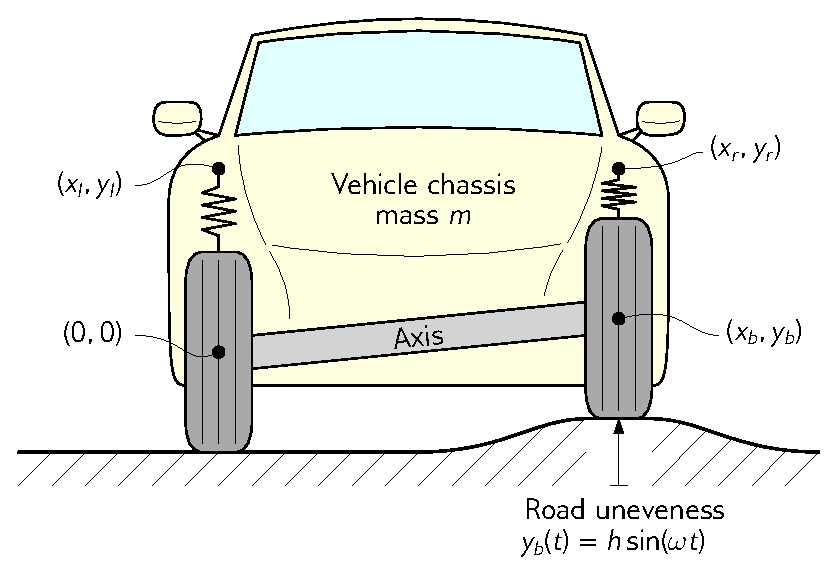
\includegraphics[width=\textwidth]{figures/car_axis.eps}
    \end{column}
  \end{columns}
  \centering{\scriptsize\begin{tabular}{cccc}
    \multicolumn{4}{c}{\textbf{Car-Axis (Index-3) -- \acs{LU} Factorization}} \\
    \toprule
    \textbf{Original \acsp{DAE}} & \multicolumn{3}{c}{$\mF = 108\cf + 131\cm + 56\ca$ \quad $\mh = 0$} \\
    \midrule
    \textbf{Reduction step} & $\mE$ & $\mg$ & $\ma$ \\
    \midrule
    Index-3 \acsp{DAE} & $12\cm$ & $94\cf + 145\cm + 54\ca$ & $14\cf + 16\cm + 10\ca$ \\
    Index-2 \acsp{DAE} & $12\cm$ & $94\cf + 145\cm + 54\ca$ & $26\cf + 45\cm + 15\ca$ \\
    Index-1 \acsp{DAE} & $12\cm$ & $94\cf + 145\cm + 54\ca$ & $136\cf + 4\cd + 261\cm + 95\ca$ \\
    Index-0 \acsp{DAE} & $1060\cf + 38\cd + 1901\cm + 717\ca$ & $431\cf + 8\cd + 842\cm + 268\ca$ & $0$ \\
    \midrule
    \rowcolor{mycolor5!25}
    \textbf{Reduced \acsp{DAE}} & \multicolumn{3}{c}{$\mF = 896\cf + 4\cd + 1202\cm + 546\ca$ \quad $\mh = 176\cf + 4\cd + 322\cm + 120\ca$} \\
    \bottomrule \\[0.05em]
    %
    \multicolumn{4}{c}{\textbf{Car-Axis (Index-3) -- \acs{FFLU} Factorization}} \\
    \toprule
    \textbf{Original \acsp{DAE}} & \multicolumn{3}{c}{$\mF = 108\cf + 131\cm + 56\ca$ \quad $\mh = 0$} \\
    \midrule
    \textbf{Reduction step} & $\mE$ & $\mg$ & $\ma$ \\
    \midrule
    Index-3 \acsp{DAE} & $0$ & $94\cf + 8\cd + 150\cm + 54\ca$ & $14\cf + 21\cm + 10\ca$ \\
    Index-2 \acsp{DAE} & $0$ & $94\cf + 8\cd + 154\cm + 54\ca$ & $26\cf + 1\cd + 44\cm + 15\ca$ \\
    Index-1 \acsp{DAE} & $0$ & $94\cf + 8\cd + 155\cm + 54\ca$ & $136\cf + 6\cd + 4\cd + 261\cm + 95\ca$ \\
    Index-0 \acsp{DAE} & $1066\cf + 55\cd + 1888\cm + 717\ca$ & $431\cf + 18\cd + 851\cm + 268\ca$ & $0$ \\
    \midrule
    \rowcolor{mycolor2!25}
    \textbf{Reduced \acsp{DAE}} & \multicolumn{3}{c}{$\mF = 1549\cf + 73\cd + 2765\cm + 1011\ca$ \quad $\mh = 176\cf + 7\cd + 326\cm + 120\ca$} \\
    \bottomrule
  \end{tabular}}
\end{frame}

\begin{frame}{Application Fields and Performance}{Expression Swell}
  \begin{columns}
    \centering
    \begin{column}[c]{0.7\textwidth}
      \hic{And when strong expression swell arise \dots}
    \end{column}
    \begin{column}[c]{0.22\textwidth}
      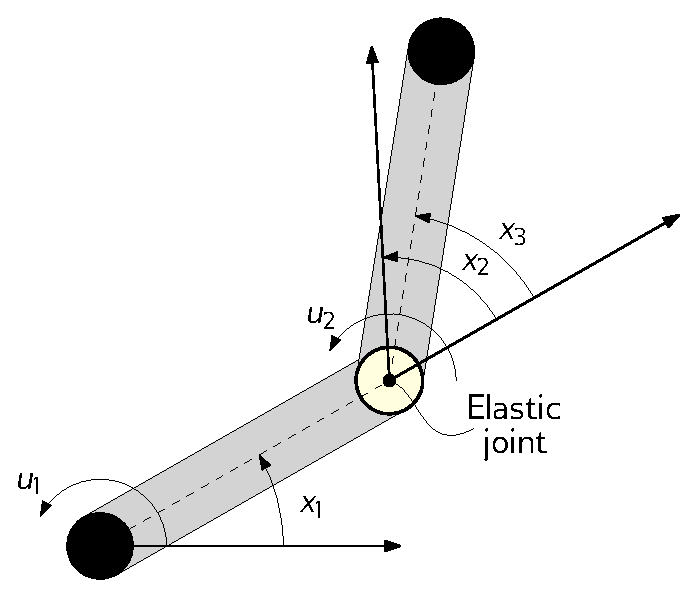
\includegraphics[width=\textwidth]{figures/robotic_arm.eps}
    \end{column}
  \end{columns}
  \hspace{-0.5em}
  \centering{\scriptsize\begin{tabular}{cccc}
    \multicolumn{4}{c}{\textbf{Robotic Arm (Index-5)}} \\
    \toprule
    \textbf{Original \acsp{DAE}} & \multicolumn{3}{c}{$\mF = 125\cf + 19\cd + 56\cm + 64\ca$ \quad $\mh = 0$} \\
    \midrule
    \textbf{Reduction step} & $\mE$ & $\mg$ & $\ma$ \\
    \midrule
    Index-5 \acsp{DAE} & $0$ & $66\cf + 3\cd + 50\cm + 35\ca$ & $16\cf + 12\ca$ \\
    Index-4 \acsp{DAE} & $0$ & $66\cf + 3\cd + 50\cm + 35\ca$ & $24\cf + 6\cm + 14\ca$ \\
    Index-3 \acsp{DAE} & $0$ & $66\cf + 3\cd + 50\cm + 35\ca$ & $162\cf + 2\cd + 138\cm + 114\ca$ \\
    Index-2 \acsp{DAE} & $14\cf + 2\cd + 6\cm + 6\ca$ & $372\cf + 4\cd + 375\cm + 253\ca$ & $972\cf + 1\cd + 1062\cm + 770\ca$ \\
    \rowcolor{mycolor2!25}
    Index-1 \acsp{DAE} & $14\cf + 2\cd + 6\cm + 6\ca$ & $372\cf + 4\cd + 375\cm + 253\ca$ & $\star (6.5\cf + 5.6\cm + 1.8\ca)\!\cdot\!10^{6} + 4\cd$ \\
    \rowcolor{mycolor2!25}
    Index-0 \acsp{DAE} & $\star (8.3\cf + 7.1\cm + 2.3\ca)\!\cdot\!10^{7} + 58\cd$ & $(2.4\cf + 2.0\cm + 0.9\ca)\!\cdot\!10^{6} + 8\cd$ & $0$ \\
    \midrule
    \rowcolor{mycolor2!25}
    \textbf{Reduced \acsp{DAE}} & \multicolumn{3}{c}{$\star \mF = (8.6\cf + 7.3\cm + 2.4\ca)\!\cdot\!10^{7} + 66\cd$ \quad $\star \mh = (6.5\cf + 5.6\cm + 1.8\ca)\!\cdot\!10^{6} + 7\cd$} \\
    \bottomrule
    \end{tabular}}
\end{frame}

\begin{frame}{Application Fields and Performance}{Expression Swell Mitigation}
  \vspace{-2.0em}
  \hic{\dots hierarchical representation does the job}
  \vspace{-0.5em}
  \centering{\scriptsize\begin{tabular}{cccc}
    \multicolumn{4}{c}{\textbf{Robotic Arm (Index-5)}} \\
    \toprule
    \textbf{Original \acsp{DAE}} & \multicolumn{3}{c}{$\mFv = 125\cf + 19\cd + 56\cm + 64\ca$ \quad $\mhv = 0$ \quad $\mv = 0$} \\
    \midrule
    \textbf{Reduction step} & $\mEv$ & $\mgv$ & $\mav$ \\
    \midrule
    Index-5 \acsp{DAE} & $0$ & $66\cf + 3\cd + 50\cm + 35\ca$ & $16\cf + 12\ca$ \\
    Index-4 \acsp{DAE} & $0$ & $66\cf + 3\cd + 50\cm + 35\ca$ & $24\cf + 6\cm + 14\ca$ \\
    Index-3 \acsp{DAE} & $0$ & $66\cf + 3\cd + 50\cm + 35\ca$ & $162\cf + 2\cd + 138\cm + 114\ca$ \\
    Index-2 \acsp{DAE} & $14\cf + 2\cd + 6\cm + 6\ca$ & $66\cf + 1\cv + 3\cd + 51\cm + 35\ca$ & $1\cm + 1\cv$ \\
    \rowcolor{mycolor5!25}
    Index-1 \acsp{DAE} & $2\cv + 1\ca$ & $66\cf + 1\cv + 3\cd + 51\cm + 35\ca$ & \cellcolor{mycolor5!25}$9\cf + 4\cv + 2\cd + 8\cm + 5\ca$ \\
    \rowcolor{mycolor5!25}
    Index-0 \acsp{DAE} & $7\cv + 1\cd + 2\cm + 2\ca$ & \cellcolor{mycolor5!25}$66\cf + 2\cv + 3\cd + 52\cm + 35\ca$ & $0$ \\
    \midrule
    \rowcolor{mycolor5!25}
    \textbf{Reduced \acsp{DAE}} & \multicolumn{3}{c}{$\mFv = 90\cf + 9\cv + 4\cd + 63\cm + 48\ca$ \quad $\mhv = 202\cf + 5\cv + 4\cd + 141\cm + 130\ca$} \\
    \bottomrule \\[-0.65em]
  \end{tabular}}
  \begin{columns}
    \centering
    \begin{column}[c]{0.5\textwidth}
      \centering{\scriptsize\begin{tabular}{cc}
        \multicolumn{2}{c}{Hierarchical representation details (29 veils)} \\
        \toprule
        \textbf{Reduction step} & $\mv$ \\
        \midrule
        Index-5 \acsp{DAE} & $0$ \\
        Index-4 \acsp{DAE} & $0$ \\
        Index-3 \acsp{DAE} & $0$ \\
        Index-2 \acsp{DAE} & $1278\cf + 3\cv + 6\cd + 1319\cm + 918\ca$ \\
        \rowcolor{mycolor3!25}
        Index-1 \acsp{DAE} & $8401\cf + 20\cv + 24\cd + 9451\cm + 6095\ca$ \\
        \rowcolor{mycolor3!25}
        Index-0 \acsp{DAE} & $37010\cf + 558\cv + 56\cd + 45087\cm + 28665\ca$ \\
        \midrule
        \rowcolor{mycolor3!25}
        \textbf{Reduced \acsp{DAE}} & $\mv = 37010\cf + 558\cv + 56\cd + 45087\cm + 28665\ca$ \\
        \bottomrule
      \end{tabular}}
    \end{column}
    \hspace{1.0em}
    \begin{column}[c]{0.215\textwidth}
      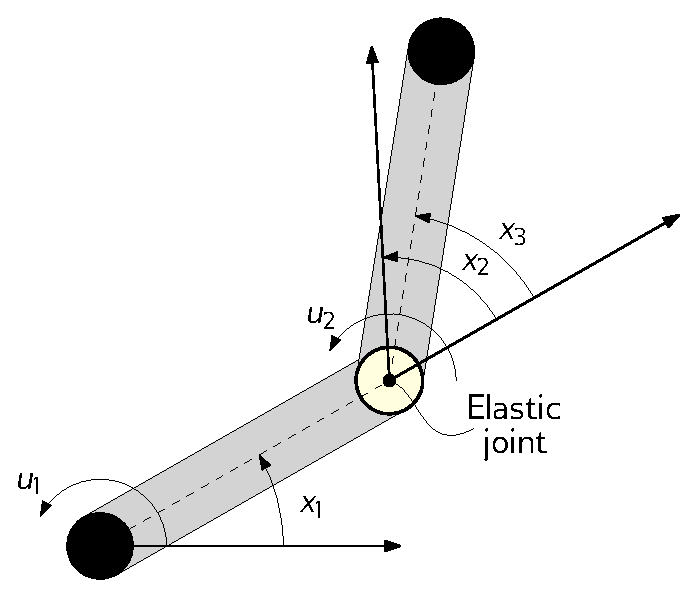
\includegraphics[width=\textwidth]{figures/robotic_arm.eps}
    \end{column}
  \end{columns}
\end{frame}

\begin{frame}{Application Fields and Performance}{Numerical Stability}
  \vspace{-2.0em}\begin{columns}
    \centering
    \begin{column}[c]{0.3\textwidth}
      \hic{Numerical\vphantom{y} stability is preserved but not guaranteed}
      \includegraphics[width=\textwidth]{figures/fade_overview.png}
    \end{column}
    \begin{column}[c]{0.7\textwidth}
      \vspace{1em}\small{\input{figures/suspension_pista_azzurra.tex}}
    \end{column}
  \end{columns}
\end{frame}

% That's all Folks!
%!TEX root = main.tex

\section{Conclusions and Future Work}

\begin{frame}{Future Work}{Critical Analysis and Perspectives}
\end{frame}

\begin{frame}{Conclusions}{Developed Software Tools}
  \Maple{} package for managing large symbolic expressions \dots
  \begin{itemize}
    \item \textbf{custom implementation} of the \Maple{}s' \texttt{LargeExpressions} package.
    \item \textbf{object-oriented} implementation for managing large symbolic expressions;
    \item \textbf{better control} over the hierarchical representation of expressions.
  \end{itemize}
  %
  \begin{bbox}[Large Expression Management \Maple{} package]
    The LEM implementation is freely available on GitHub! \\
    \centering \url{https://github.com/StoccoDavide/LEM}
  \end{bbox}
\end{frame}

\begin{frame}{%
  Symbolic Computation Methods for the Numerical \\
  Solution of Dynamic Systems Described by \\
  Differential-Algebraic Equations
  }{Davide Stocco}
  \vfill
  \raggedright{\fontfamily{qag}\selectfont\Huge\color{tx_sl_color}\bfseries{Thank you for your attention!}} \\[0.5em]
  \raggedleft{\fontfamily{qag}\selectfont\Huge\color{tx_sl_color}\bfseries{Questions?}}
\end{frame}

% That's all Folks!
\appendix
%!TEX root = main.tex

\begin{frame}{Q1 -- Gerdts}
  Is there a connection between the tractability index and the construction of projectors therein and the procedure using LU decompositions in Chapter 4?
\end{frame}

\begin{frame}{Q2 -- Gerdts}
  How does the developed symbolic factorization method compare to GENDA by Mehrmann/Kunkel in view of CPU times?
\end{frame}

\begin{frame}{Q3 -- Gerdts}
  The minimum degree pivoting strategy apperantly worked for the examples in the thesis. In general, I assume, it cannot guarantee that all pivots are non-zero during evaluation. If a zero pivot is detected for a specific example, how would you proceed with the symbolic factorization?
\end{frame}

\begin{frame}{Q4 -- Gerdts}
  Is it necessary to reduce to index-0 or would it be sufficient to reduce to index-1 and use a standard integrator like DASSL, RADAUIIA?
\end{frame}

\begin{frame}{Q1 -- Mazzia}
  Usually, there is no information related to all initial conditions, which must be calculated consistently. Do you think the index reduction strategy can be used to calculate consistent initial values?
\end{frame}

\begin{frame}{Q2 -- Mazzia}
  How does the developed symbolic factorization method compare to GENDA by Mehrmann/Kunkel in view of CPU times?
\end{frame}

% That's all Folks!
%%!TEX root = main.tex

\section{The Implemented Symbolic Matrix Factorization}

\begin{frame}{Symbolic Matrix Factorization}{\acf{LU}}
  \begin{bbox}[Full-Pivoting \acs{LU} Factorization]
    Given a matrix $\m{A} \in \mathbb{R}^{m \times n}$, with $m \geq n$, the full-pivoting \acs{LU} decomposition is defined as the process of decomposing $\m{A}$ into the product of
    \begin{itemize}
      \item a $\m{L} \in \mathbb{R}^{m \times m}$ lower-triangular matrix with all diagonal entries equal to $1$
      \item a $\m{U} \in \mathbb{R}^{m \times n}$ upper-triangular matrix
      \item a $\m{P} \in \mathbb{R}^{m \times m}$ and a $\m{Q} \in \mathbb{R}^{n \times n}$ matrices for rows and columns permutation
    \end{itemize}
    such that $\m{P}\m{A}\m{Q} = \m{L}\m{U}$
  \end{bbox}
\end{frame}

\begin{frame}{Symbolic Matrix Factorization}{\acf{FFLU}}
  \begin{bbox}[Full-Pivoting \acs{FFLU} Factorization]
    Given a matrix $\m{A} \in \mathbb{R}^{m \times n}$, with $m \geq n$, the full-pivoting \acs{FFLU} decomposition is defined as the process of decomposing $\m{A}$ into the product of
    \begin{itemize}
      \item a lower-triangular matrix $\m{L} \in \mathbb{R}^{m \times m}$ with all diagonal entries equal to $1$;
      \item \textcolor{fg_sl_color}{a diagonal matrix $\m{D} \in \mathbb{R}^{m \times m}$}
      \item an upper-triangular matrix $\m{U} \in \mathbb{R}^{m \times n}$
      \item a $\m{P} \in \mathbb{R}^{m \times m}$ and a $\m{Q} \in \mathbb{R}^{n \times n}$ matrices for rows and columns permutation
    \end{itemize}
    such that $\m{P}\textcolor{fg_sl_color}{\m{D}}\m{A}\m{Q} = \m{L}\m{U}$
  \end{bbox}
\end{frame}

\section{A Symbolic Approach to Structure Compliance}

\begin{frame}{A Symbolic Approach to Structure Compliance}{Practical Application on Vehicle Suspension Compliance
  Analysis}
  \begin{minipage}[c]{0.6\textwidth}
    \begin{itemize}
      \item The suspension system has to \textbf{guarantee} \dots
      \begin{enumerate}
        \item \textbf{comfort} to the passengers{minimize vertical accelerations of the chassis}
        \item \textbf{road holding} and \textbf{stability} of the vehicle
        \item control the \textbf{wheel attitude} with respect to the road surface
      \end{enumerate}
      \hspace{0.5cm}
\begin{tikzpicture}
        \draw[fg_sl_color, ultra thick,-stealth] (0,0) |- (0.5,-1) node[anchor=west] {\hi{Flexibility affects the vehicle dynamics}};
      \end{tikzpicture}
    \end{itemize}
  \end{minipage}
  \begin{minipage}[c]{0.35\textwidth}
    \includegraphics[width=1.0\textwidth]{car_suspension.png}
  \end{minipage}
\end{frame}

\begin{frame}{K\&C analysis}{Introduction}
  \begin{minipage}[c]{0.55\linewidth}
    The \textbf{kinematics} and \textbf{compliance} of the suspension system are \dots
    \begin{enumerate}
      \item the \textbf{motion} and \textbf{deformation} of the system
      \item key aspects of the \textbf{design} of the system \vspace*{1.0em}
    \end{enumerate}
    \begin{center}\begin{minipage}{6.0cm}\begin{block}{}
      \centering
      \hi{Kinematics and compliance are what is needed to describe the suspension in a vehicle model}
    \end{block}\end{minipage}\end{center}
  \end{minipage}
  \hfill
  \begin{minipage}[c]{0.4\linewidth}
    \centering
    \vspace{-2.0em}
    \includegraphics[width=1.0\linewidth]{kinematic_model.png} \\[-4em]
    \hspace*{-10em}
    \includegraphics[width=0.7\linewidth, trim={9cm 0cm 0cm 0cm}, clip]{compliance_model.pdf}
  \end{minipage}
\end{frame}

\begin{frame}{K\&C analysis}{State-of-the-art solutions}
  \begin{center}
    \begin{tabular}{lcccc}
      \toprule
      \textbf{Methods} & \textbf{Real-Time} & \textbf{Accuracy} & \textbf{Parametric} & \textbf{Easy to Setup} \\
      \midrule
      FE methods & \mycrossmark & \mycheckmark & \mycrossmark  & \mycrossmark \\
      Map-based methods & \mycheckmark & \mydotmark & \mycrossmark & \mycheckmark \\
      Flexible multibody & \mydotmark & \mycheckmark & \mydotmark & \mycrossmark \\
      What we aim to \dots & \mycheckmark & \mydotmark & \mycheckmark & \mycheckmark \\
      \bottomrule
    \end{tabular}
  \end{center}
  \vspace{0.5cm}
  \begin{center}
    \emph{Legend}: \mycheckmark{} satisfied, \mydotmark{} satisfied with limitations, and \mycrossmark{} not satisfied.
  \end{center}
\end{frame}

\begin{frame}{Symbolic computation}{Finite element method problem}
  \begin{itemize}
    \item Symbolic computation can be applied to the \textbf{finite element (FE) method}. \\
    \item \textbf{Stiffness matrix}, \textbf{load vector}, and \textbf{boundary conditions} are defined symbolically. \\
    \begin{equation*}
      \begin{bmatrix}
        \mathbf{K}_{ff} & \mathbf{K}_{fs} \\
        \mathbf{K}_{sf} & \mathbf{K}_{ss}
      \end{bmatrix} \begin{bmatrix}{c}
        \mathbf{d}_{f} \\
        \mathbf{d}_{s}
      \end{bmatrix} = \begin{bmatrix}{c}
        \mathbf{f}_{f} \\
        \mathbf{f}_{s}
      \end{bmatrix}
      \quad \xrightarrow[\text{method}]{\text{direct stiffness}} \quad
      \begin{array}{c}
        \mathbf{d}_{f} = \mathbf{K}_{ff}^{-1}\,\left(\mathbf{f}_{f} - \mathbf{K}_{fs}\,\mathbf{d}_{s}\right) \\
        \mathbf{f}_{s} = \mathbf{K}_{sf}\,\mathbf{d}_{f} + \mathbf{K}_{ss}\,\mathbf{d}_{s}
      \end{array}
    \end{equation*}
    \begin{enumerate}
      \item Possibility to \textbf{evaluate} the system \textbf{without} the need to ``\textbf{reassemble}'' the system \\
      \item Parametric formulation \\
      \item Symbolic solution of the structure deformations and reaction forces \\
    \end{enumerate}
  \end{itemize}
  \begin{center}\begin{minipage}{10.75cm}\begin{block}{}
    \centering
    FE method $\quad \xrightarrow[\text{computation}]{\text{symbolic}} \quad$ Symbolic FE model + \textcolor{mycolor5}{\textbf{A lot of flexibility!}}
  \end{block}\end{minipage}\end{center}
  \begin{itemize}
    \item We combined all these features in the \Maple{} \TrussMe{} library (open-source)
  \end{itemize}
\end{frame}

\begin{frame}{Symbolic computation}{Linear algebra}
  \begin{itemize}
    \item Symbolic matrix factorization is used for the computation of the linear system \textbf{solutions}
    \begin{equation*}
      \mathbf{d}_{f} = \mathbf{K}_{ff}^{-1}\,\left(\mathbf{f}_{f} - \mathbf{K}_{fs}\,\mathbf{d}_{s}\right)
    \end{equation*}
    \begin{bbox}[Problem]
      \Maple matrix factorizations have \textbf{limited capabilities}.
    \end{bbox}
    \item We developed the \texttt{LAST} symbolic matrix factorization toolbox capable of \dots  \\
    \begin{enumerate}
      \item extending \Maple factorization capabilities \\
      \item introducing \textbf{veiling variables} not to increase the expressions size (through \texttt{LEM} toolbox) \\
      \item performing efficient LU, Fraction-Free LU, QR, and Gauss-Jordan factorizations with limited \textbf{expresion swell} \\
    \end{enumerate}
  \end{itemize}
\end{frame}

\begin{frame}{Symbolic computation}{Mixed symbolic/numerical solution}
  \begin{itemize}
    \item \textbf{Symbolic} solution is not always possible due to
    \begin{enumerate}
      \item capability of the symbolic kernel to handle \textbf{complicated} expressions
      \item \textbf{non-linear} or mathematically \textbf{unsolvable} problems
    \end{enumerate}
     \item Symbolic computation should be exploited as much as possible!
  \end{itemize}
  \begin{center}\begin{minipage}{1.0\textwidth}\begin{block}{}
    \centering
    FE model $\quad \xrightarrow[\text{computation}]{\text{symbolic}} \quad$ \hspace*{1.05cm}\textcolor{mycolor2}{\textbf{Stop}}\hspace*{1.05cm} $\quad \xrightarrow[\text{generation}]{\text{code}} \quad$ \begin{minipage}[c]{0.27\linewidth}\begin{center}{\textbf{Efficient} numeric \\ FE model solution}\end{center}\end{minipage}
  \end{block}\end{minipage}\end{center}
  \begin{center}\begin{minipage}{1.0\textwidth}\begin{block}{}
    \centering
    FE model $\quad \xrightarrow[\text{computation}]{\text{symbolic}} \quad$ \textcolor{mycolor5}{\textbf{Symbolic solution}} $\quad \xrightarrow[\text{generation}] {\text{code}} \quad$ \begin{minipage}[c]{0.27\linewidth}\begin{center}{\textbf{Fastest} \\ numeric evaluation!}\end{center}\end{minipage}
  \end{block}\end{minipage}\end{center}
  \begin{itemize}
    \item K\&C{} of suspensions are computed through a \textbf{mixed} symbolic/numerical approach
  \end{itemize}
\end{frame}

\begin{frame}{Suspensions symbolic modeling}{Case study}
  The modeled suspension is a \textbf{double wishbone} suspension system of the \textbf{Formula SAE} vehicle of \emph{E-Agle Trento Racing Team} (University of Trento) \\[1.0em]
  \begin{center}
    \begin{minipage}[c]{0.65\textwidth}
      \centering
      \includegraphics[width=1.0\textwidth]{render_all.pdf}
    \end{minipage}
    \hspace*{1em}
    \begin{minipage}[c]{0.25\textwidth}
      \centering
      \includegraphics[width=1.0\textwidth]{fsae.jpeg}
    \end{minipage}
  \end{center}
\end{frame}

\begin{frame}{Suspensions symbolic modeling}{Rigid multibody \& FE models}
  \begin{minipage}[c]{0.55\linewidth}
    \includegraphics[width=0.8\textwidth]{fade_overview.png}\\
    \hi{138 DoFs symbolic FE model}
  \end{minipage}
  \begin{minipage}[c]{0.40\linewidth}
    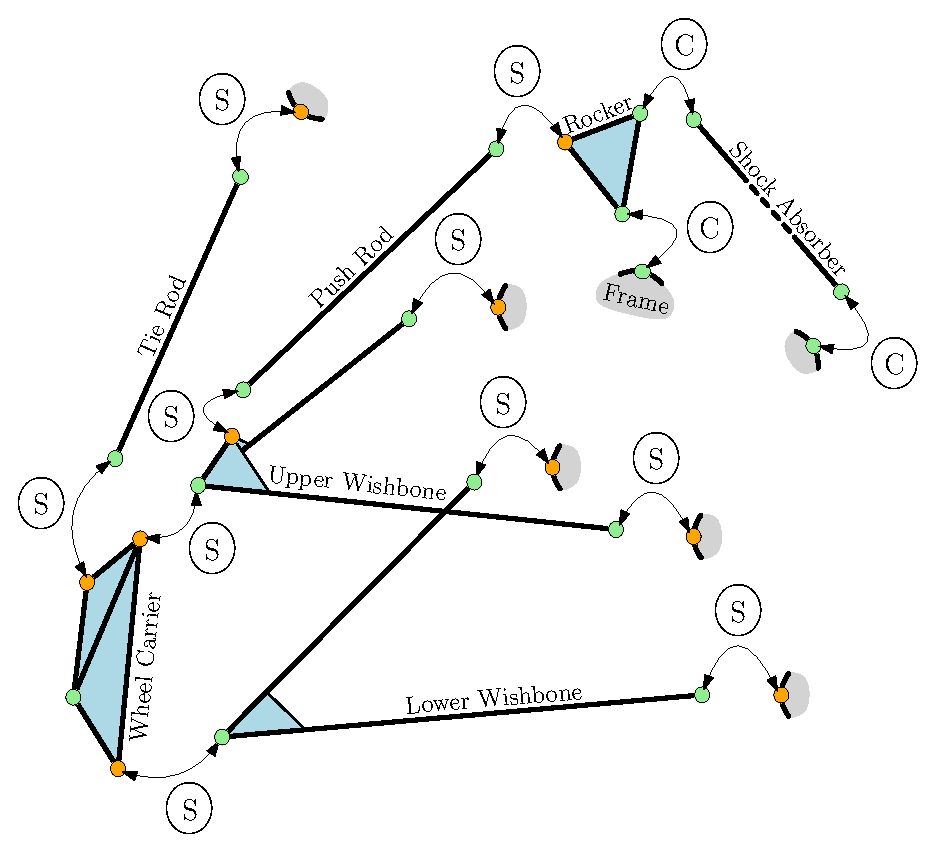
\includegraphics[width=1.0\textwidth]{constraints.eps}
  \end{minipage}
\end{frame}

\begin{frame}{Simulation results}{Static analysis}
  \vspace{-1.75em}
  \begin{center}
    \begin{minipage}[c]{0.485\linewidth}
      \centering{\textbf{Static translations}} \\[0.2em]
      \includegraphics[width=1.0\textwidth]{static_translations.pdf}
    \end{minipage}
    \begin{minipage}[c]{0.485\linewidth}
      \centering{\textbf{Static rotations}} \\[0.2em]
      \includegraphics[width=1.0\textwidth]{static_rotations.pdf}
    \end{minipage}
    \raggedright{\footnotesize{\emph{Legend:} \TrussMe{} solution (\emph{solid lines}), \Ansys{} data (\emph{bullets}). \\ {\color{mycolor1}$\blacksquare$} $F_x =$ \SI{4000}{\newton}, {\color{mycolor2}$\blacksquare$} $F_y =$ \SI{4000}{\newton}, {\color{mycolor3}$\blacksquare$} $F_z =$ \SI{4000}{\newton}, with $M_x = M_y = M_z =$ \SI{0}{\newton\meter}. \\ {\color{mycolor4}$\blacksquare$} $M_x =$ \SI{400}{\newton\meter}, {\color{mycolor5}$\blacksquare$} $M_y =$ \SI{400}{\newton\meter}, {\color{mycolor6}$\blacksquare$} $M_z =$ \SI{400}{\newton\meter}, with $F_x = F_y = F_z =$ \SI{0}{\newton}}}
  \end{center}
\end{frame}

\begin{frame}{Suspensions symbolic modeling}{Modeling assumptions}
  \begin{minipage}[t]{0.32\linewidth}
    \centering
    \hi{No compliance}\\[3.4em]
    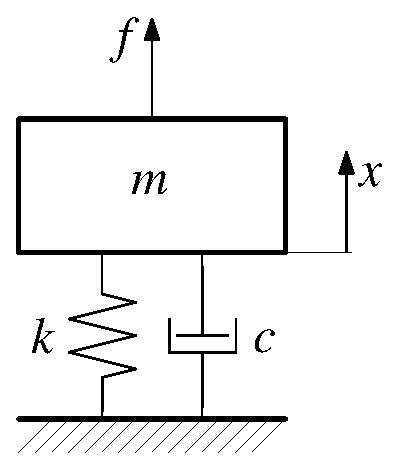
\includegraphics[width=0.5\textwidth]{system_no_compliance.eps}
    \begin{equation*}
      m \ddot{x} + c \dot{x} + k x = f
    \end{equation*}
  \end{minipage}
  \hfill
  \begin{minipage}[t]{0.32\linewidth}
    \centering
    \hi{Quasi-static compliance}\\[0.5em]
    \includegraphics[width=0.5\textwidth]{system_superposition.eps}
    \begin{equation*}
      \begin{cases}
        y = x + d  \\
        k_c d = f  \\
        m \ddot{x} + c \dot{x} + k x = f
      \end{cases}
    \end{equation*}
  \end{minipage}
  \hfill
  \begin{minipage}[t]{0.32\linewidth}
    \centering
    \hi{Dynamic compliance}\\[0.52em]
    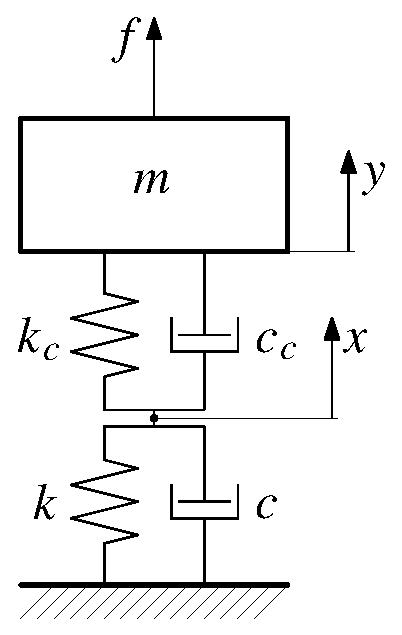
\includegraphics[width=0.5\textwidth]{system_real.eps}
    \begin{equation*}
      \begin{cases}
        y = x + d \\
        k x + c \dot{x} = k_c d + c_c \dot{d} \\
        m \ddot{y} = k_c d + c_c \dot{d} + f
      \end{cases}
    \end{equation*}
  \end{minipage}
\end{frame}

\begin{frame}{Suspensions symbolic modeling}{Frequency response}
  \centering{The \textbf{frequency response} of the system is influenced by the \textbf{decoupling} strategy.} \\[0.5em]
  \begin{columns}
    \begin{column}[c]{0.7\textwidth}
      \begin{itemize}
        \item[{\color{mycolor1}$\blacksquare$}] no compliance
          \vspace{-0.2cm}%
          {\scriptsize{
          \begin{flalign*}
          \dfrac{\ddot{Y}(s)}{F(s)} = \dfrac{s^2}{ms^2 + cs + k}&&
          \end{flalign*}
          }}
        \item[{\color{mycolor2}$\blacksquare$}] quasi-static compliance
        \vspace{-0.2cm}%
          {\scriptsize{
          \begin{flalign*}
          \dfrac{\ddot{Y}(s)}{F(s)} = \dfrac{s^2}{ms^2 + cs + k} + \dfrac{s^2}{k_c} \quad \substack{\omega_{n} = \sqrt{\dfrac{k}{m}} \\[1em] \omega_z = \sqrt{\dfrac{k + k_c}{m}}}&&
          \end{flalign*}
          }}
        \item[{\color{mycolor3}$\blacksquare$}] dynamic compliance
          \vspace{-0.2cm}%
          {\scriptsize{
          \begin{flalign*}
          \dfrac{\ddot{Y}(s)}{F(s)} = \dfrac{(c \!+\! c_c)s^3 + (k \!+\! k_c)s^2}{m(c \!+\! c_c)s^3 + (c\,c_c + m(k \!+\! k_c))s^2 + (k_c\,c \!+\! k\,c_c)s + k\,k_c}&&
          \end{flalign*}
          }}
      \end{itemize}
    \end{column}%
    \hspace{-4.5cm}%
    \begin{column}[c]{0.4\textwidth}
      \vspace{-1.0cm}
      \includegraphics[width=1.05\linewidth]{tf_theory.pdf}
    \end{column}
  \end{columns}
\end{frame}

\begin{frame}{Simulation results}{Frequency response}
  \begin{minipage}[c]{0.69\linewidth}
    \centering{\textbf{Acceleration/force frequency response}} \\[0.25em]
    {\footnotesize{
    \includegraphics[width=0.8\textwidth]{frequency_tz.pdf}
    \begin{center}
      \emph{Legend:}
      {\color{mycolor1}$\blacksquare$} MB with compliance dynamic, {\color{mycolor2}$\blacksquare$} MB and steady-state compliance, {\color{mycolor3}$\blacksquare$} \Ansys \ac{FE} modal analysis.
    \end{center}
    }}
  \end{minipage}
  \hfill
  \begin{minipage}[c]{0.3\linewidth}
    \includegraphics[width=0.5\linewidth]{mode1.png} \raisebox{2.0em}{\small{$f = 7.6$ Hz}} \\
    \includegraphics[width=0.5\linewidth]{mode2.png} \raisebox{2.0em}{\small{$f = 88.5$ Hz}} \\
    \includegraphics[width=0.5\linewidth]{mode3.png} \raisebox{2.0em}{\small{$f = 159.7$ Hz}} \\
  \end{minipage}
\end{frame}

\begin{frame}{Simulation results}{Full Vehicle Simulation}
  \begin{columns}
  \begin{column}{0.55\textwidth}
    \includegraphics[width=0.95\textwidth]{compliance_PA.pdf}\\
    \emph{Legend}: {\color{mycolor1}$\blacksquare$} $x$-, {\color{mycolor2}$\blacksquare$} $y$-, {\color{mycolor3}$\blacksquare$} $z$-component.
  \end{column}
  \begin{column}{0.47\textwidth}
    \includegraphics[width=1.0\textwidth]{kine_compliance_PA.pdf}\\
    \emph{Legend}: {\color{mycolor1}$\blacksquare$} kinematic, {\color{mycolor2}$\blacksquare$} total.
  \end{column}
  \end{columns}
\end{frame}

\begin{frame}{Simulation results}{Timing}
  \begin{center}
  \begin{table}[ht]
    \centering
    \begin{tabular}{p{0.3\textwidth}ccccc}
      \toprule
      \textbf{Compliance} & \multicolumn{4}{c}{\textbf{Computation time}} \\ \cmidrule(l{5pt}r{5pt}){2-5}
      \textbf{model} & $\mu$\,(\si{\micro\second}) & $\min$\,(\si{\micro\second}) & $\max$\,(\si{\micro\second}) & $\sigma^2$\,(\si{\micro\second\squared}) \\
      \midrule
      Compliance maps (linear) & $\phantom{0}40$ & $\phantom{0}4$ & $\phantom{0}48$ & $\phantom{0}1.2$ \\
      Compliance maps (cubic)  & $193$           & $84$           & $880$           & $42.9$ \\
      Symbolic FEM             & $181$           & $42$           & $417$           & $45.2$ \\
      \bottomrule
    \end{tabular}
  \end{table}
\end{center}
\end{frame}

\section{Tire-Road Interaction Modelling}

\begin{frame}{Geometry Library}
  \vspace{-1.0em}%
  \centering%
  \begin{minipage}[c]{0.45\textwidth}%
    \centering\def\svgwidth{6.5cm}%
    \small{\input{figures/acme_entities_1.pdf_tex}} \\
    \def\svgwidth{6.5cm}%
    \small{\input{figures/acme_entities_2.pdf_tex}}
  \end{minipage}%
  \hfill%
  \begin{minipage}[c]{0.45\textwidth}%
    \centering\def\svgwidth{6.5cm}%
    \small{\input{figures/acme_collection.pdf_tex}}
  \end{minipage}%
\end{frame}

\begin{frame}{Tire-Road Interaction Model}
  \vspace{-1.0em}
  \centering
  \includegraphics[width=0.3\textwidth]{zoom_ipe.pdf}%
  \includegraphics[width=0.35\textwidth]{intersection.pdf} \\
  \includegraphics[width=0.3\textwidth]{tire_zoom.pdf}%
  \includegraphics[width=0.5\textwidth]{road_shell_ipe.pdf}
\end{frame}

\begin{frame}{Tire-Road Interaction Model}
  \vspace{-1.0em}
  \centering
  \includegraphics[width=0.6\textwidth]{steps.pdf}%
  \includegraphics[width=0.4\textwidth]{rtf_enve.pdf}
\end{frame}

\begin{frame}{Brush Tire Model}
  \vspace{-1.0em}
  \centering
  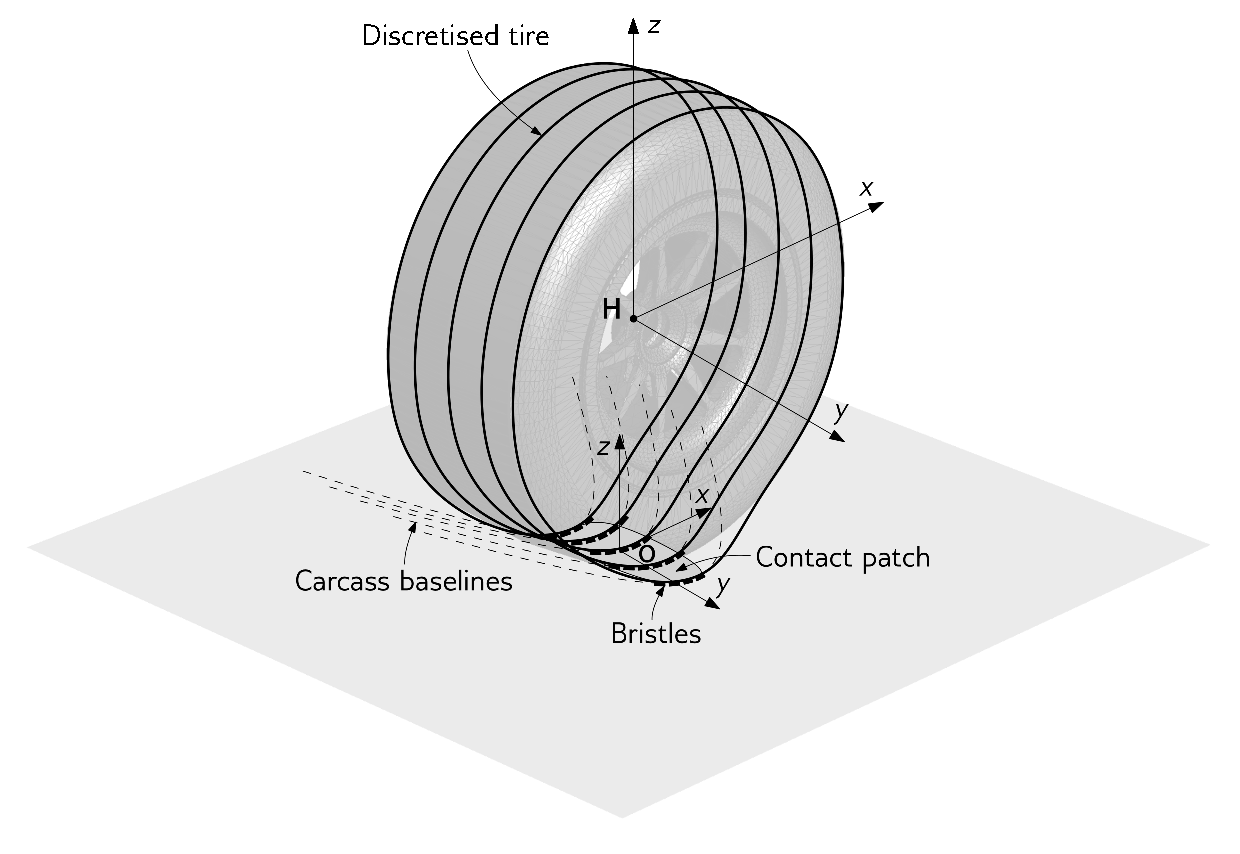
\includegraphics[width=0.75\textwidth]{brush_model.eps}
\end{frame}

\begin{frame}{Brush Tire Model}
  \vspace{-1.0em}
  \centering
  \includegraphics[width=0.475\textwidth]{fx_tire.pdf}%
  \includegraphics[width=0.475\textwidth]{fy_tire.pdf} \\
  \includegraphics[width=0.475\textwidth]{mz_tire.pdf}
\end{frame}

\begin{frame}{Brush Tire Model}
  \vspace{-1.0em}
  \centering
  \small{\begin{tabularx}{0.8\textwidth}{*{6}{Y}}%{\textwidth}{*{14}{Y}}
    %\multicolumn{14}{c}{\textbf{Quasi-Newton Methods Performance with 5 Ribs}} \\
    \multicolumn{6}{c}{\textbf{Quasi-Newton Methods Performance with 5 Ribs}} \\
    \toprule
    \multirow{2.25}{*}{\textbf{Method}} &
    %\multicolumn{4}{c}{\textbf{Evaluations} ($-$)} &
    %\multicolumn{4}{c}{\textbf{Iterations} ($-$)} &
    \multicolumn{4}{c}{\textbf{Time} (\USI{\micro\second})} &
    \multirow{2}{*}{\textbf{Success}} \\
    \cmidrule(l{4pt}r{4pt}){2-5}
    %\cmidrule(l{4pt}r{4pt}){6-9}
    %\cmidrule(l{4pt}r{4pt}){10-13}
    %& \mini{} & \maxi{} & \meai{} & \vari{} & \mini{} & \maxi{} & \meai{} & \vari{}
      & \mini{} & \maxi{} & \meai{} & \vari{} & \\
    \midrule
    PIM   %& $100$ & $100$ & $100.0$ & $0.00$    & $100$ & $100$ & $100.0$ & $0.0$
      & $518.0$ & $7949.0$ & $617.2$  & $13953.2$  & $0.0\%$   \\ %\hline
    G1M   %& $-$   & $-$   & $-$     & $-$       & $-$   & $-$   & $-$     & $-$
      & $-$     & $-$      & $-$      & $-$        & Overflow  \\ %\hline
    G2M   %& $4$   & $100$ & $9.2$   & $55.8$    & $4$   & $100$ & $9.2$   & $55.8$
      & $23.5$  & $1089.4$ & $69.0$   & $5252.0$   & $99.5\%$  \\ %\hline
    ENM   %& $6$   & $200$ & $11.9$  & $234.0$   & $3$   & $100$ & $6.5$   & $58.5$
      & $25.0$  & $2025.0$ & $81.5$   & $11002.8$  & $99.4\%$  \\ %\hline
    BBM   %& $-$   & $-$   & $-$     & $-$       & $-$   & $-$   & $-$     & $-$
      & $-$     & $-$      & $-$      & $-$        & $0.0\%$   \\ %\hline
    BGM   %& $4$   & $100$ & $8.8$   & $18.4$    & $4$   & $100$ & $8.8$   & $18.4$
      & $22.6$  & $948.1$  & $62.5$   & $1973.0$   & $99.9\%$  \\ %\hline
    BCM   %& $4$   & $17$  & $8.4$   & $6.7$     & $4$   & $17$  & $8.4$   & $6.7$
      & $22.9$  & $264.4$  & $55.7$   & $885.9$    & $100.0\%$ \\ %\hline
    D-PIM %& $100$ & $496$ & $190.7$ & $13628.1$ & $100$ & $100$ & $100.0$ & $0.0$
      & $507.0$ & $5383.0$ & $1151.9$ & $568491$   & $0.0\%$   \\ %\hline
    D-G1M %& $-$   & $-$   & $-$     & $-$       & $-$   & $-$   & $-$     & $-$
      & $-$     & $-$      & $-$      & $-$        & Overflow  \\ %\hline
    D-G2M %& $4$   & $376$ & $11.3$  & $572.4$   & $4$   & $100$ & $9.3$   & $57.1$
      & $21.5$  & $3195.5$ & $80.4$   & $40321.9$  & $99.5\%$  \\ %\hline
    D-ENM %& $6$   & $513$ & $12.8$  & $829.7$   & $3$   & $100$ & $6.3$   & $44.3$
      & $27.0$  & $5207.7$ & $97.5$   & $52752.6$  & $99.5\%$  \\ %\hline
    D-BBM %& $4$   & $125$ & $11.0$  & $58.0$    & $4$   & $42$  & $9.3$   & $12.8$
      & $22.3$  & $1284.0$ & $76.9$   & $5126.3$   & $100.0\%$ \\ %\hline
    D-BGM %& $4$   & $376$ & $9.7$   & $110.6$   & $4$   & $100$ & $8.7$   & $15.1$
      & $21.3$  & $3238.9$ & $67.0$   & $8142.9$   & $99.9\%$  \\ %\hline
    D-BCM %& $4$   & $35$  & $9.1$   & $14.6$    & $4$   & $17$  & $8.4$   & $6.7$
      & $22.5$  & $316.8$  & $62.1$   & $1615.1$   & $100.0\%$ \\
    \bottomrule
  \end{tabularx}}%
\end{frame}

\begin{frame}{Brush Tire Model}
    \vspace{-1.0em}
    \centering
    \small{\begin{tabularx}{0.75\textwidth}{*{6}{Y}}%{\textwidth}{*{14}{Y}}
    %\multicolumn{14}{c}{\textbf{Broyden Combined Method Performance}} \\
    \multicolumn{6}{c}{\textbf{Broyden Combined Method Performance}} \\
    \toprule
    \multirow{2.25}{*}{\textbf{Ribs}} &
    %\multicolumn{4}{c}{\textbf{Evaluations} ($-$)} &
    %\multicolumn{4}{c}{\textbf{Iterations} ($-$)} &
    \multicolumn{4}{c}{\textbf{Time} (\USI{\micro\second})} &
    \multirow{2}{*}{\textbf{Success}} \\
    \cmidrule(l{4pt}r{4pt}){2-5}
    %\cmidrule(l{4pt}r{4pt}){6-9}
    %\cmidrule(l{4pt}r{4pt}){10-13}
    %\multirow{0.5}{*}{\textbf{of Ribs}}
    %& \mini{} & \maxi{} & \meai{} & \vari{} & \mini{} & \maxi{} & \meai{} & \vari{}
      & \mini{} & \maxi{} & \meai{} & \vari{} & \\
    \midrule
    $1$  %& $6$     & $11$    & $7.9$   & $10.3$
         %& $6$     & $11$    & $7.9$   & $10.3$
         & $12.1$  & $89.0$  & $19.4$  & $20.6$  & $100.0\%$ \\ %\hline
    $5$  %& $4$     & $17$    & $7.9$   & $10.3$
         %& $4$     & $17$    & $7.9$   & $10.3$
         & $22.9$  & $264.4$ & $55.7$  & $885.9$ & $100.0\%$ \\ %\hline
    $10$ %& $6$     & $11$    & $7.9$   & $10.3$
         %& $6$     & $11$    & $7.9$   & $10.3$
         & $106.9$ & $361.8$ & $167.3$ & $1746.22$ & $100.0\%$ \\ %\hline
    $15$ %& $6$     & $11$    & $7.9$   & $10.3$
         %& $6$     & $11$    & $7.9$   & $10.3$
         & $158.0$ & $523.5$ & $249.4$ & $3878.2$ & $100.0\%$ \\ %\hline
    $20$ %& $6$     & $11$    & $7.9$   & $10.3$
         %& $6$     & $11$    & $7.9$   & $10.3$
         & $210.1$ & $693.3$ & $332.9$ & $7028.7$ & $100.0\%$ \\ %\hline
    $25$ %& $6$     & $11$    & $7.9$   & $10.3$
         %& $6$     & $11$    & $7.9$   & $10.3$
         & $262.7$ & $858.4$ & $414.0$ & $10708.3$ & $100.0\%$ \\
    \bottomrule
  \end{tabularx}}%
\end{frame}

% That's all Folks!

\end{document}

% That's all Folks!